\section{Experiments \& Applications}
\label{sec:evaluation}
\definecolor{darkblue}{rgb}{0.0, 0.0, 0.55}
\definecolor{oxfordblue}{rgb}{0.0, 0.13, 0.28}
\newcommand{\MYhref}[3][oxfordblue]{\href{#2}{\color{#1}{#3}}}%

We examine the inferential results achieved by our method under 3 statistical models, in scenarios capturing different types of data mismatch with reality. The data contamination models used in following experiments are reminiscent of \emph{Huber's $\eps$-contamination model}~\citep{huber92}, which postulates that observed data are generated from a mixture of distributions of the form $(1-\eps)\cdot G+ \eps\cdot Q$, where $\eps \in (0,1)$,  $G$ is a distribution of inliers captured by the assumed statistical model, and $Q$ is an arbitrary distribution of outliers. This model has found use in several recent studies on robust statistical estimators suitable for underlying data distributions with minimal assumptions~\citep{wei17, chen18}.

\bcores{} is compared against a uniformly random sampling baseline, and stochastic batch implementations of two existing Riemannian coreset methods: 
\benum[label={(\roman*)}]
	\item \sparsevi~\cite{campbell19neurips}, which builds up a coreset according to an incremental scheme similar to ours, considering the standard likelihood function terms evaluated on the dataset points, and 
	\item \psvi~\cite{psvi}, which runs a batch optimization on a set of pseudopoints, and uses standard likelihood evaluations to jointly learn the pseudopoints weights and locations so that the extracted summary resembles the statistics of the full dataset. 
\eenum


We default the number of iterations in the optimization loop over gradient-based coreset constructions to $ T = 500$, using a learning rate $ \gamma_t \propto t^{-1}$ and $S=100$ random projections per gradient computation. For consistency with the compared baselines, we evaluate inference results obtained by \bcores{} using the classical Bayesian posterior from~\cref{eq:bayes-rule} conditioned on the corresponding robustified data summary. Additional details on used benchmark datasets are presented in~\cref{sec:data-details}. Code is available at 	\MYhref{https://github.com/dionman/beta-cores}{https://github.com/dionman/beta-cores}.

\subsection{Simulated Gaussian Mean Inference under Stuctured Data Contamination}
\label{subsec:gauss-expt}

In this experiment we study how \bcores{} behaves in the setting of mean inference on synthetic $d$-dimensional data, sampled \iid from a normal distribution with known covariance,
\[
\theta \sim \distNorm\left(\mu_0, \Sigma_0\right),
\qquad 
\;\;\;\;\;
x_n \distiid \distNorm(\theta, \Sigma),
\qquad
n = 1, \ldots, N.
\label{eq:mvn-expt}
\]
In the presented results, we use priors $\mu_0=\mathbf{0}$ and $\Sigma_0=I$,  dimensionality $d=20$ and dataset size $N=5,000$.
 
We consider the case of structured data corruption existing in the observations, simulated as follows: Observed datapoints are typically sampled from a Gaussian $ \distNorm(\mathbf{1}, I)$. At a percentage $F\%$,  data collection fails; in this case, datapoints are collected from a shifted Gaussian $ \distNorm(\mathbf{10}, I)$. Consequently, the observed dataset forms a Gaussian mixture with two components; however, our statistical model assumes only a single Gaussian.

All computations involved in the coreset construction and posterior evaluation in this experiment can be performed in closed form~\cite{campbell19neurips}. We apply the batch scheme of~\cref{alg:bcores}, sampling from the exact coreset posterior over gradient estimation. The used \mbox{($\beta$-)}likelihood equations are outlined in~\cref{sec:gauss-lik}. For all coreset methods, constructions are repeated for up to $M=200$ iterations, with $\gamma_t = t^{-1}$. Notice that our setting does not imply that maximum summary size contains 200 datapoints: often over the iterations an already existing summary point may be selected again, resulting in smaller coresets.


\begin{figure}[t!]
	\centering 
	\begin{subfigure}[b]{0.9\textwidth} 
		\includegraphics[width=1.\textwidth]{\MyPath/figs/gauss_scatterplot.png}
		\caption{\label{fig:beta_gaussian_coreset_points}}
	\end{subfigure}
	\hfill\qquad
	\begin{subfigure}[b]{0.9\textwidth} 
		\centering
		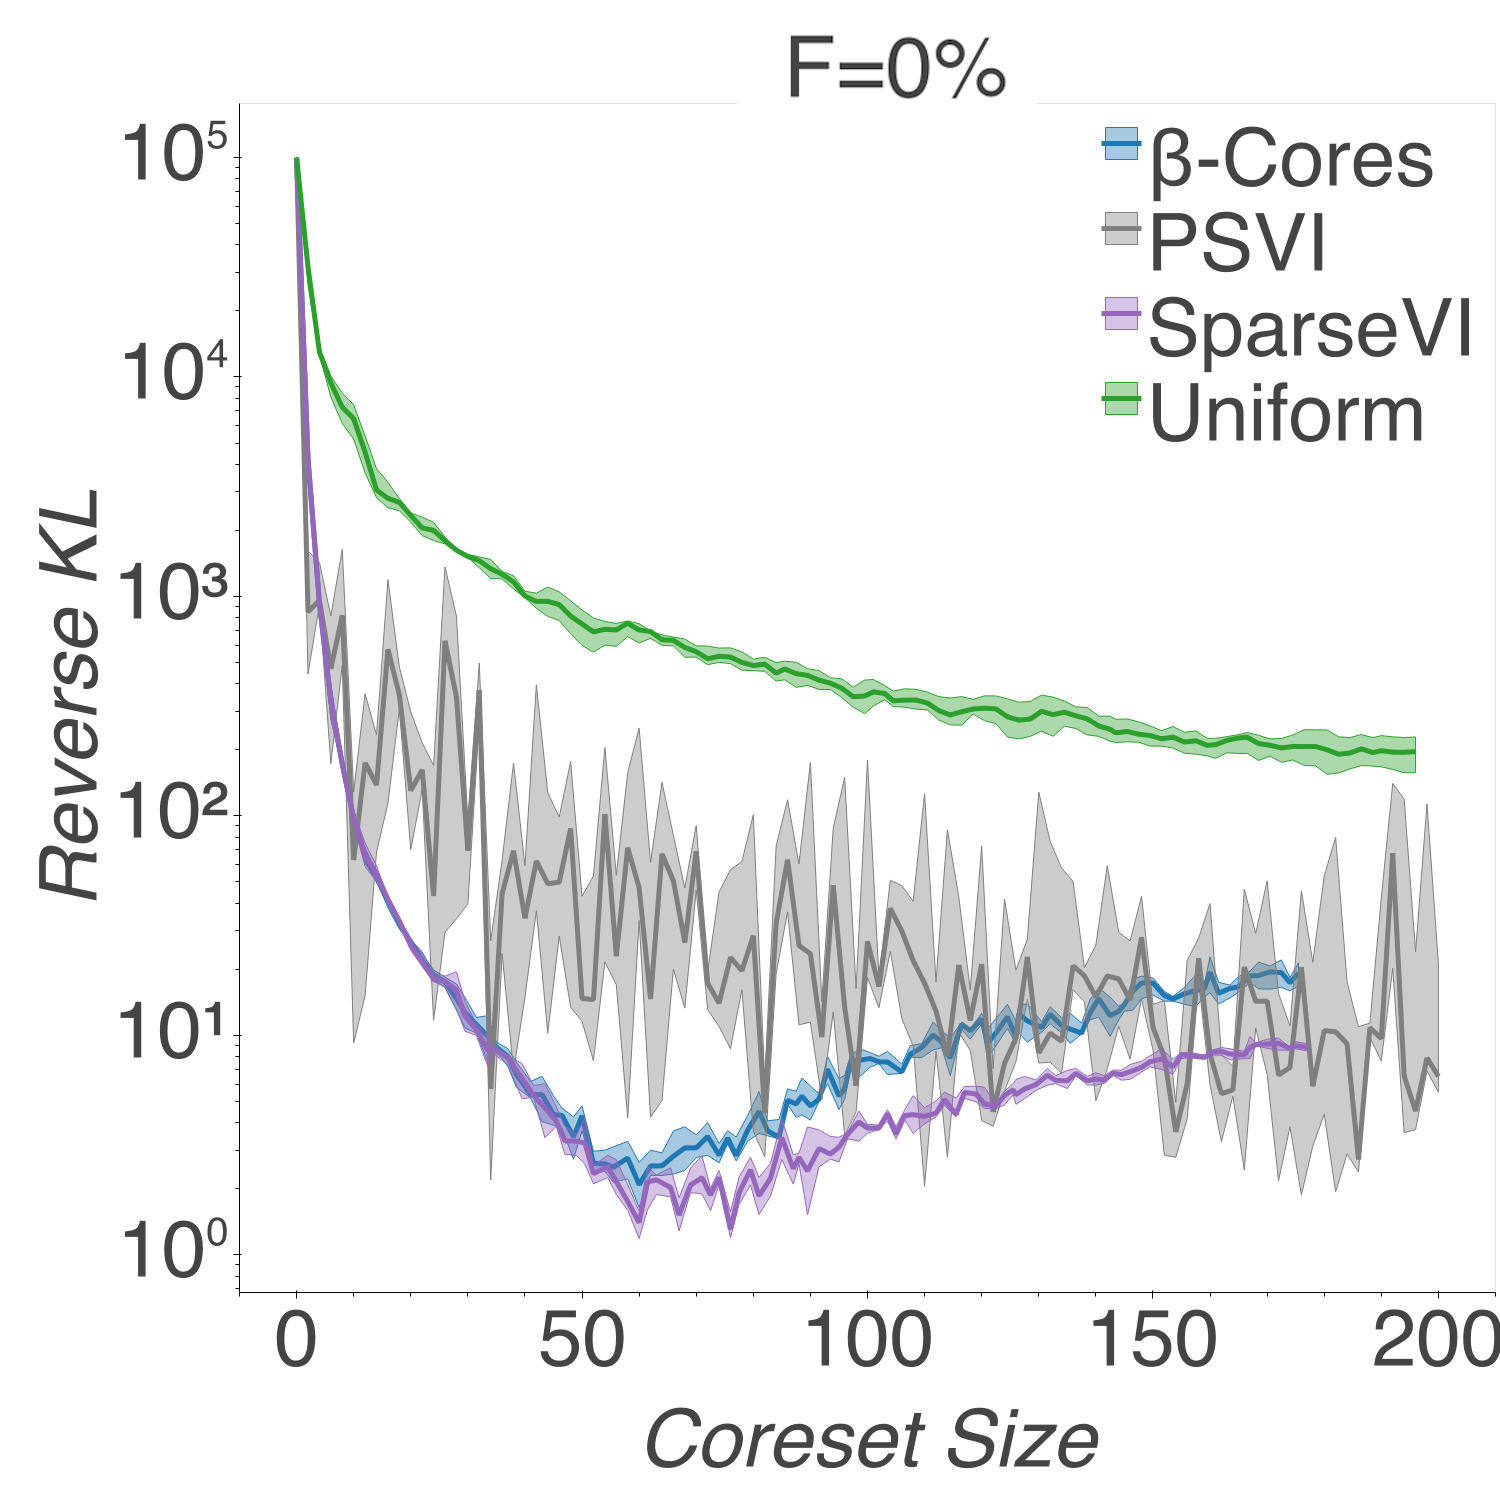
\includegraphics[width=.3\textwidth]{\MyPath/figs/f0KLDvsCstSize.png}
		\centering
		\hfill
		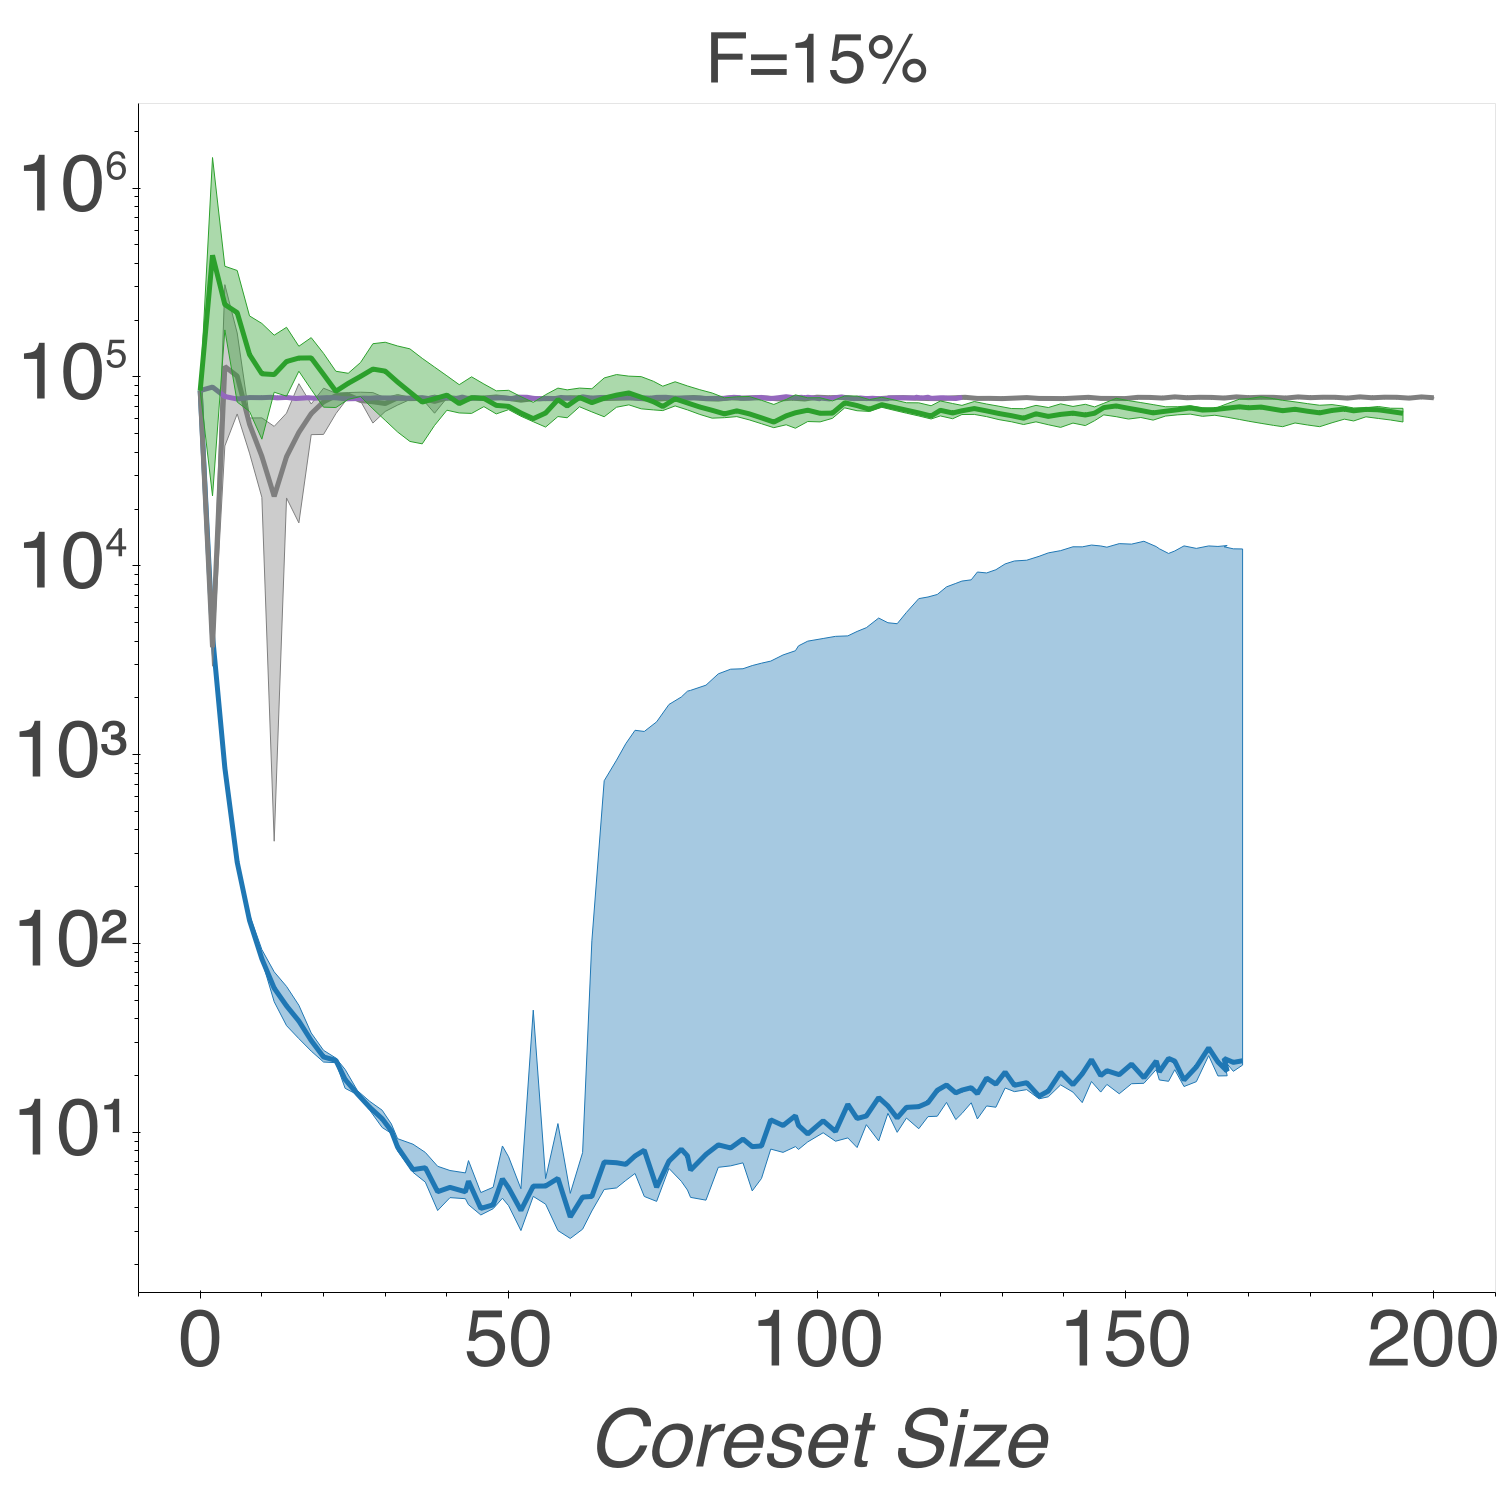
\includegraphics[width=.3\textwidth]{\MyPath/figs/f15KLDvsCstSize.png}
		\centering
		\hfill
		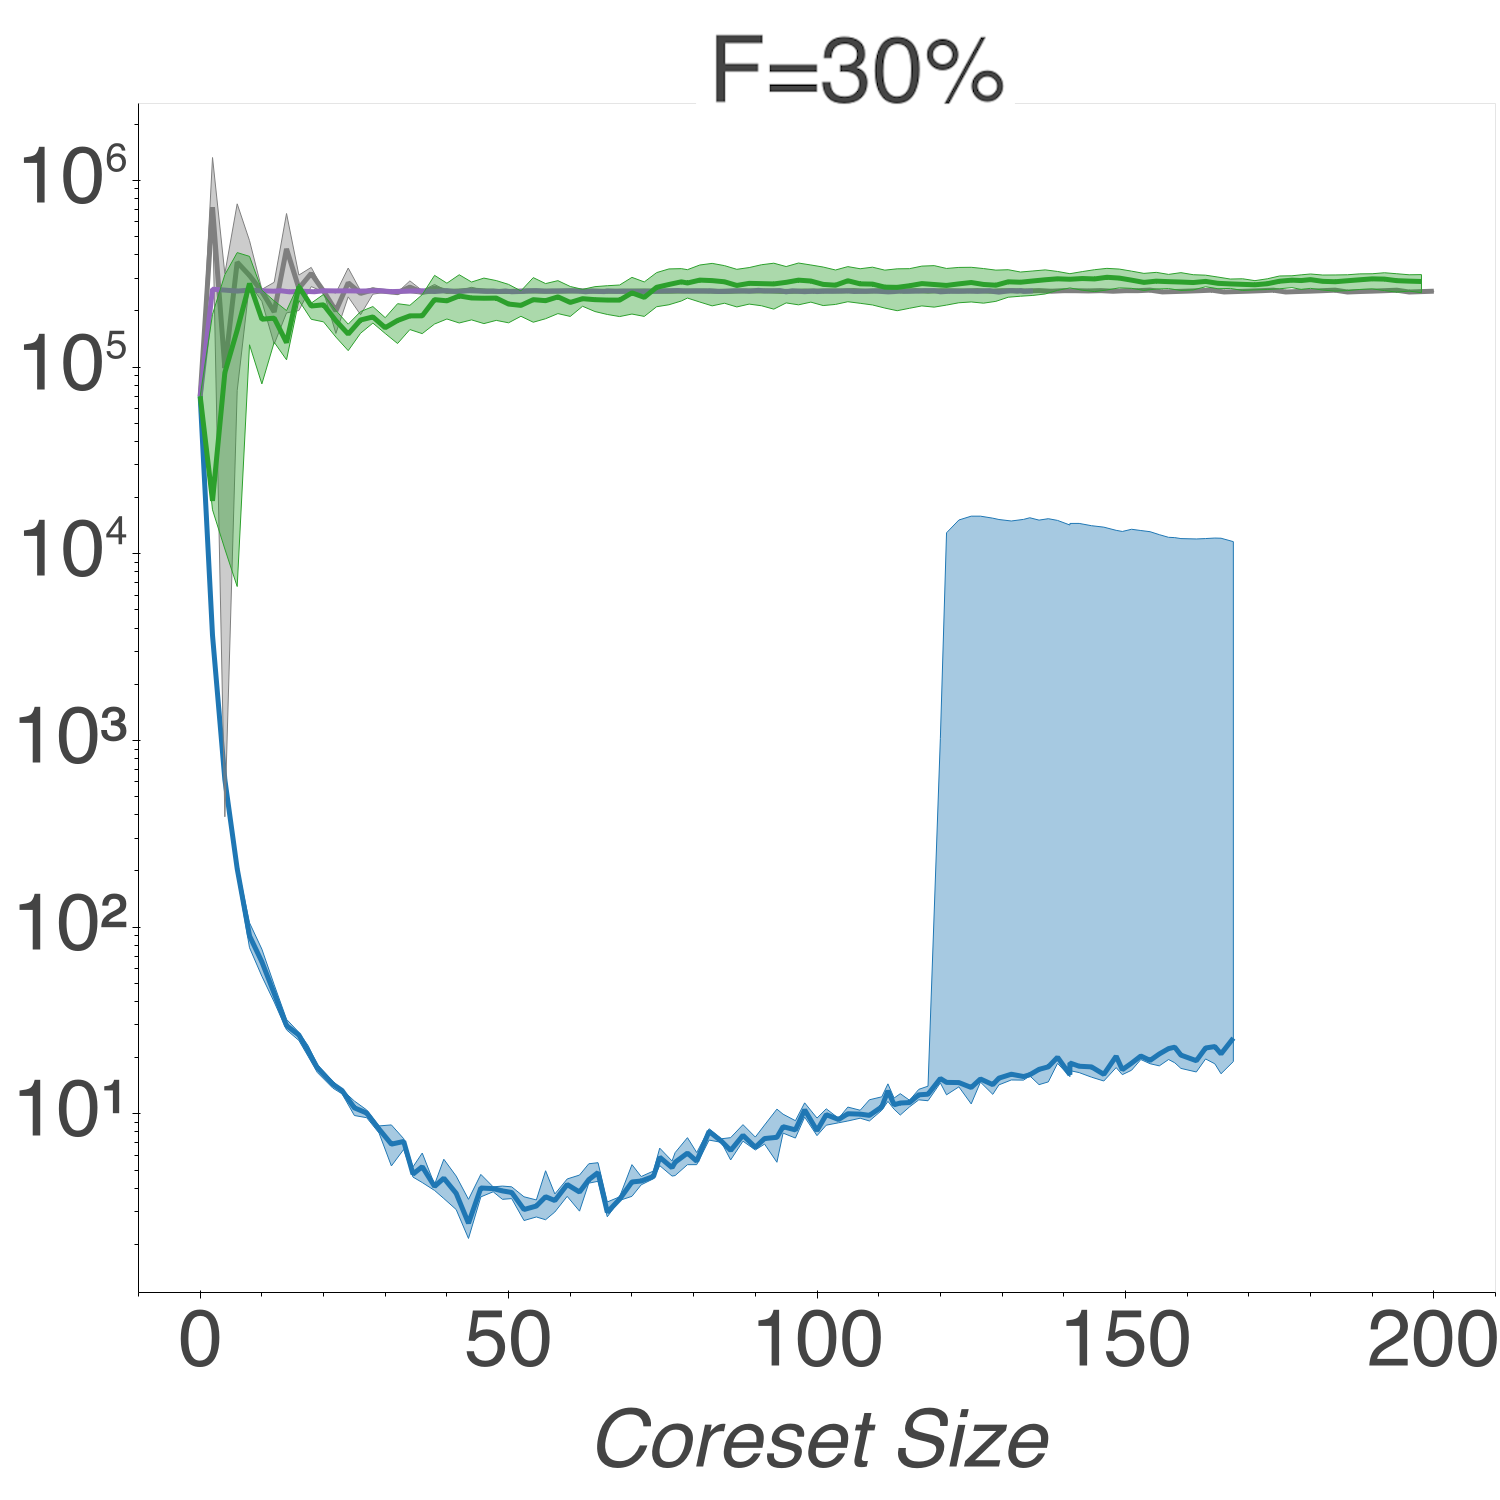
\includegraphics[width=.3\textwidth]{\MyPath/figs/f30KLDvsCstSize.png}
		\caption{\label{fig:gauss_kld}}
	\end{subfigure}	
	\centering
	\caption{(a)~Scatterplot of the observed datapoints projected on two random axes, overlaid by the corresponding coreset points and predictive posterior $3\sigma$ ellipses for increasing coreset size (from left to right). Exact posterior (illustrated in black) is computed on the dataset after removing the group of outliers. From top to bottom, the level of structured contamination increases. Classical Riemannian coresets are prone to model misspecification, adding points from the outlying component, while \bcores{} adds points only from the uncontaminated subpopulation yielding better posterior estimation. (b) Reverse KL divergence between coreset and true posterior, averaged over $5$ trials. Solid lines display the median KL divergence, with shaded areas showing $25\textsuperscript{th}$ and $75\textsuperscript{th}$ percentiles of KL divergence.}
\end{figure}


\cref{fig:beta_gaussian_coreset_points}~presents the results obtained by the different coreset methods. We stress-test their performance under varying amounts of data corruption~(from top to bottom, 0\%, 15\%, and 30\% of the datapoints get replaced by outliers). We can verify that \bcores{} with $\beta=0.01$ is on par with existing Riemannian coresets in an uncontaminated dataset. Noticeably, \bcores{} remains robust to high levels of structured corruption~(even up to $30\%$ of the dataset), giving reliable posterior estimates; KL divergence plots in~\cref{fig:gauss_kld} reconfirm the superiority of inference via~\bcores{}. On the other hand, in the presence of outliers, previous Riemannian coresets performance degrades quickly, offering similar posterior inference quality with random sampling. The KL divergence from the cleansed data posterior for existing summarizations and uniform sampling increases with observations failure probability, as it asymptotically converges to the Bayesian posterior computed on the corrupted dataset. 

Moreover, in the case of contaminated datasets, baseline coresets are quite confident in their wrong predictive posteriors: they keep assigning the same weight to all observations and hence do not adjust their posterior uncertainty estimates, in spite of having to describe contradicting data. In contrast,~\bcores{} discards samples from the outlying group and can confidently explain the inliers, despite the smaller effective sample size: indeed,~\cref{fig:gauss_kld} shows that the achieved KL divergence from the exact posterior is at same order of magnitude regardless of failure probability. 

We can however notice that, for coreset sizes growing beyond 60 points---despite remaining consistently better compared to the baselines---\bcores{} starts to present some instability over trials in contaminated dataset instances. This effect is attributed to the small value of the $\beta$ hyperparameter  selected for the demonstration (so that this value can successfully model the case of clean data). As a result, eventually some outliers might be allowed to enter the summary for large coreset sizes. The instability can be resolved by increasing $\beta$ according to the observations failure probability. 


\subsection{Bayesian Logistic Regression under Mislabeling and Feature Noise}
\label{subsec:logreg-expt}


In this section, we study the robustness achieved by~\bcores{} on the problem of binary classification  under unreliable measurements and labeling. We test our methods on 3 benchmark datasets with varying dimensionality~($10$-$127$ dimensions, more details on the data are provided in~\cref{sec:data-details}). We observe data pairs $(x_n, y_n)_{n=1}^{N}$, where $x\in\reals^{d}$, $y_n \in \{-1,1\}$, and use the Bayesian logistic regression model to describe them,
\[
y_n | x_n, \theta \sim \distBern \left( \frac{1}{1+e^{-z_n^T \theta}}\right),
\qquad 
z_n:=\begin{bmatrix}
x_n \\
1
\end{bmatrix}.
\]
\blik{} terms required in our construction are computed in~\cref{sec:logreg-lik}. 

Data corruption is simulated by generating outliers in the input and output space similarly to~\cite{futami18}: For corruption rate $F$, we sample two random subsets of size $F\cdot N$ from the training data.  For the datapoints in the first subset, we replace the value of half of the features with Gaussian noise sampled \iid from $\distNorm(0,5)$; for the datapoints in the other subset, we flip the binary label. Over construction we use Laplace approximation~\cite{mackay03} to efficiently draw samples from the (non-conjugate) coreset posterior, while over evaluation coreset posterior samples are obtained via NUTS~\cite{hoffman14}. We evaluate accuracy over the test set, predicting labels according to the maximum log-likelihood rule under the posterior $\theta$ sampling distribution. Learning rate schedule was set to $\gamma_t=c_0 t^{-1}$, with $c_0$ set to 1 for \sparsevi{} and \bcores{}, and 0.1 for \psvi. %~in \textsc{Phishing} and \textsc{WebSpam} datasets, 
The values for hyperparameter $\beta$ and learning rates $\gamma_t$ were chosen via cross-validation. 

\cref{fig:logreg_plot} illustrates that \bcores{} shows competitive performance with the classic Riemannian coresets in the absence of data contamination~(bottom row), while it consistently achieves the best predictive accuracy in corrupted datasets~(top row).  On the other hand, ordinary summarization techniques, although overall outperforming random sampling for small coreset sizes, soon attain degraded predictive performance on poisoned data: by construction, via increasing coreset size, Riemannian coresets are expected to converge to the Bayesian posterior computed on the corrupted dataset. All baselines present noticeable degradation in their predictive accuracy when corruption is introduced (typically more than $5\%$), which is not the case for our method: \bcores{} is designed to support corrupted input and, for a well-tuned hyperparameter $\beta$, maintains similar performance in the presence of outliers, while practically it can even achieve improvement (as occurring for the \textsc{WebSpam} data).
%\footnote{For~\textsc{WebSpam} we notice that coresets performance in uncontaminated data for the displayed summary sizes is comparable to uniform sampling: this is a side effect of the high-dimensionality of this dataset examined in more depth at~\citep{psvi}, which out of scope for the purposes of this work.},


\begin{figure}[t!]
	\begin{subfigure}[b]{0.9\textwidth} 
		\centering
		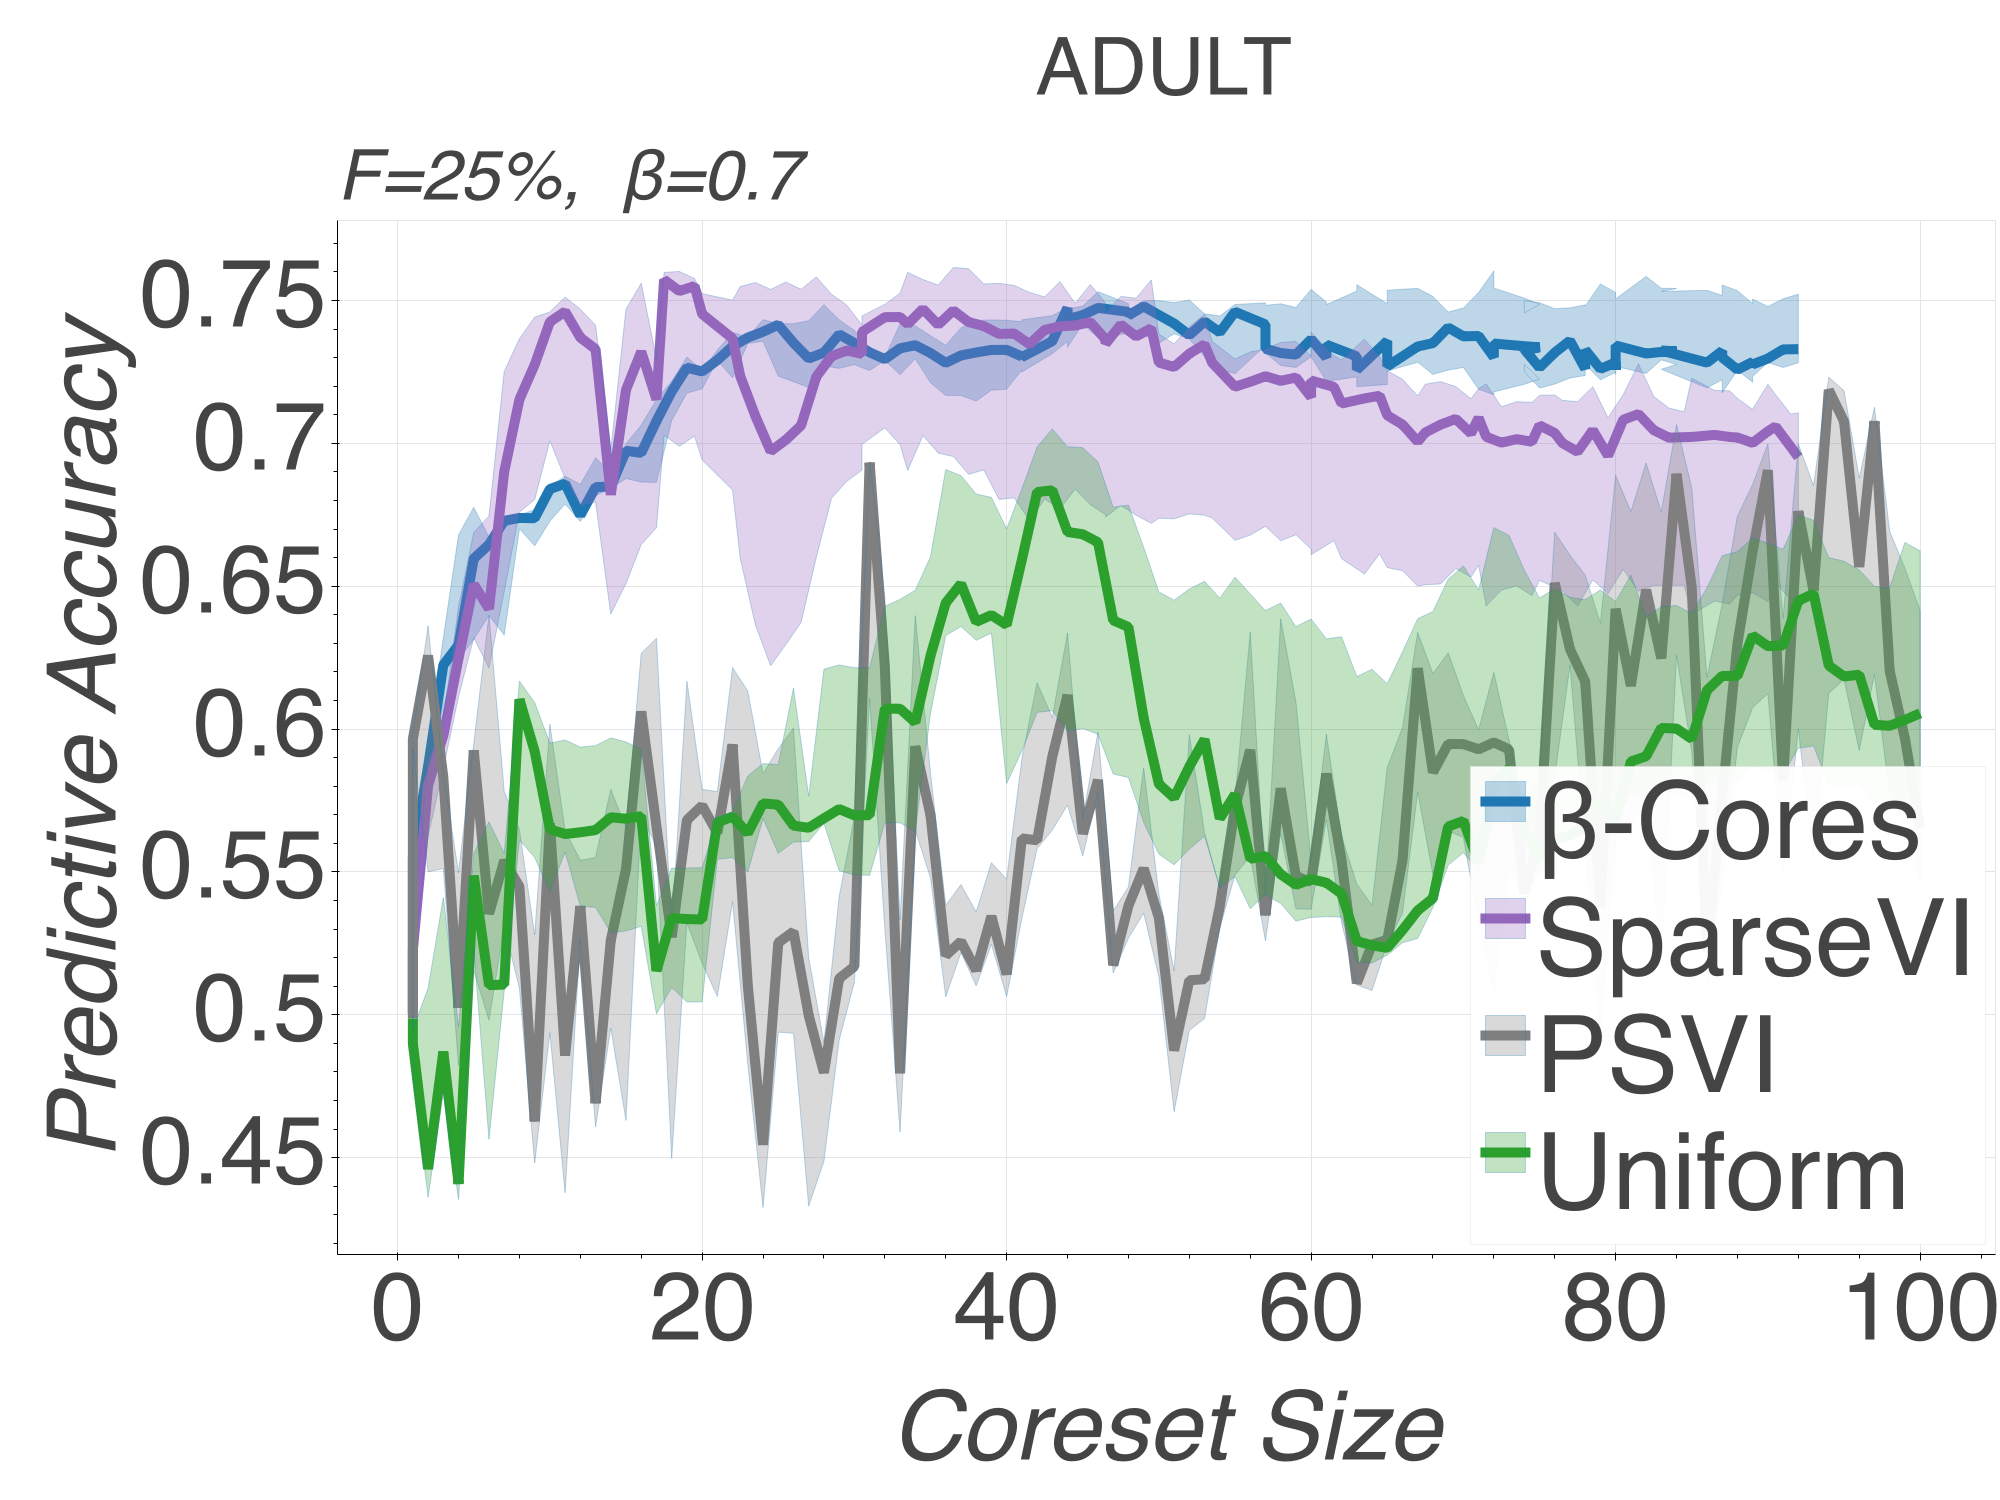
\includegraphics[width=.325\textwidth]{\MyPath/figs/adult07_10_25_False_False_ACCvssz.png}
		\centering
		\hfill
		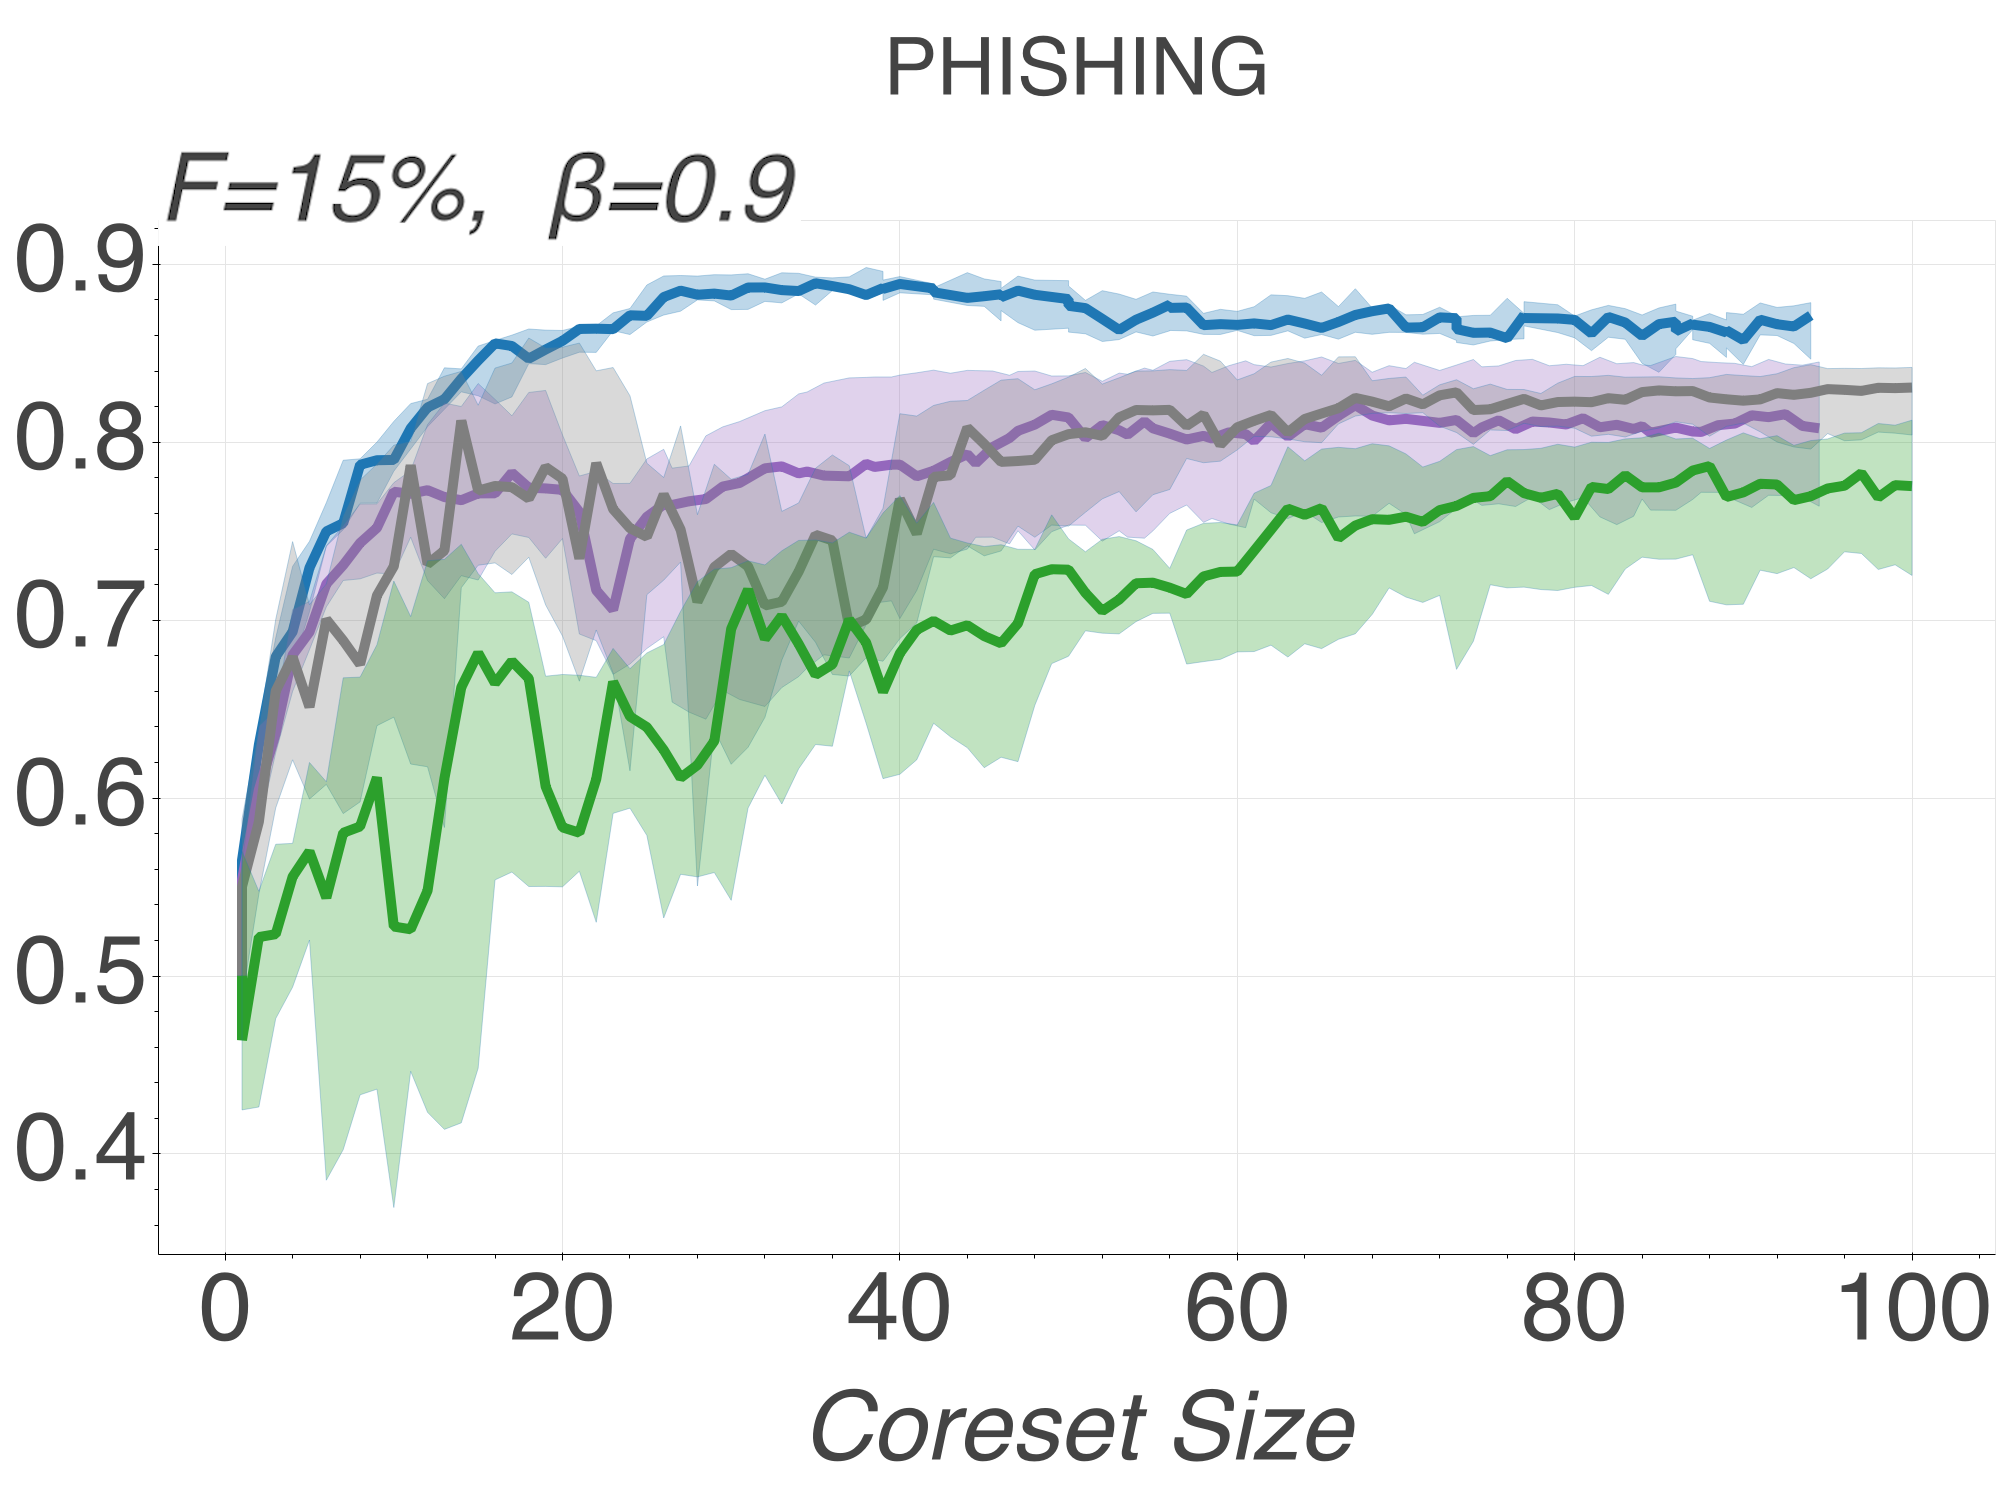
\includegraphics[width=.325\textwidth]{\MyPath/figs/phish09_10_15_False_False_ACCvssz.png}
		\centering
		\hfill
		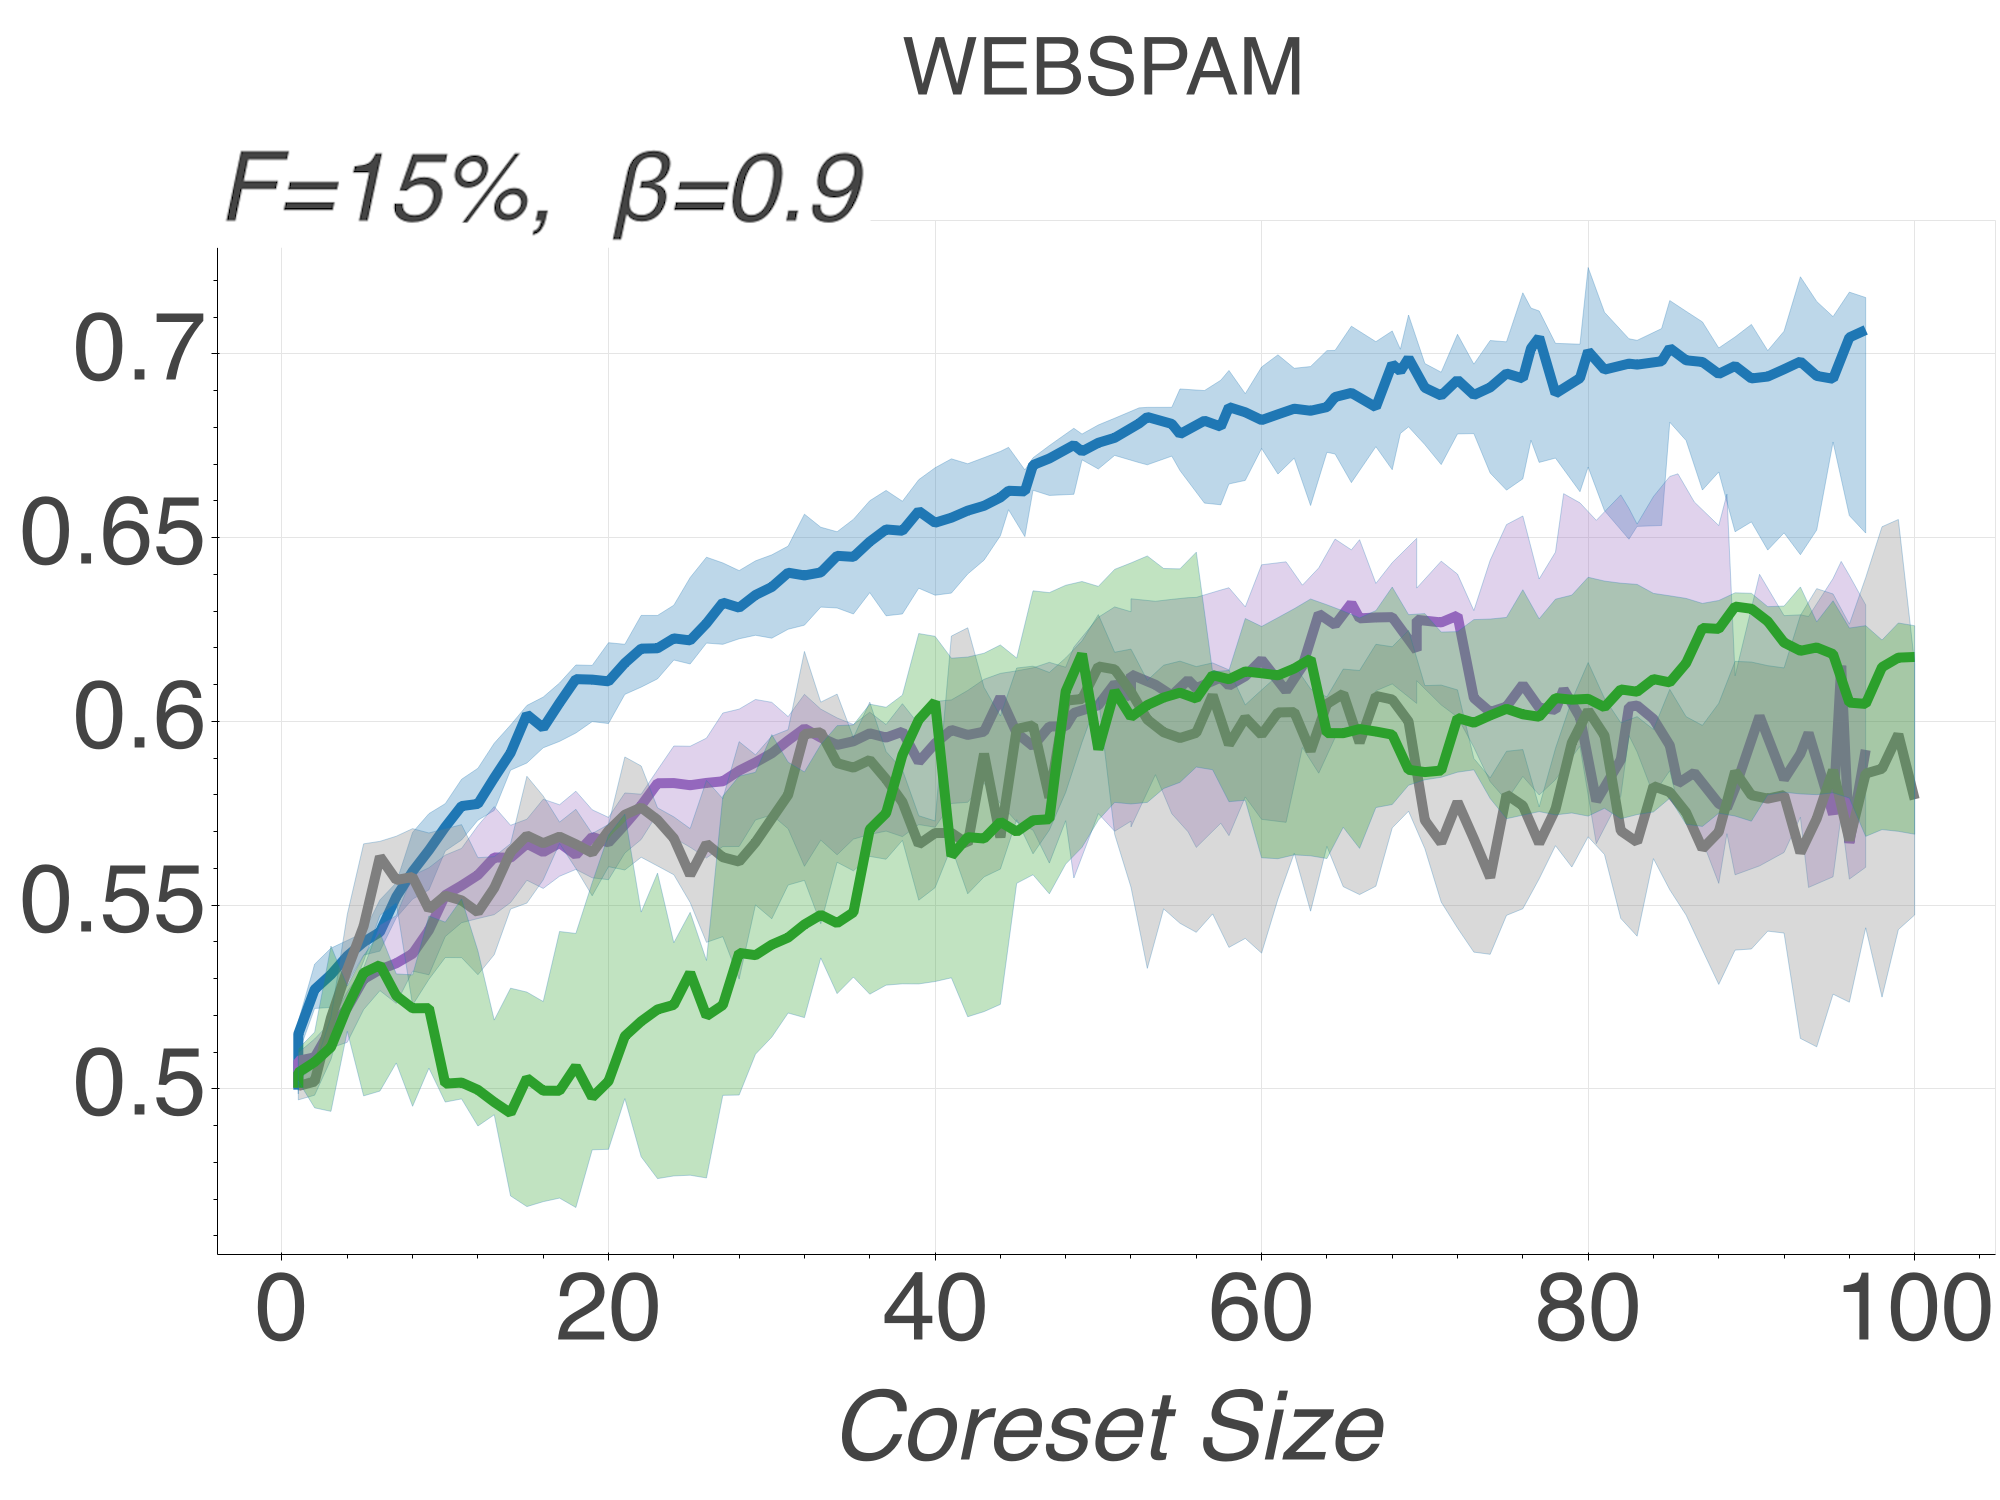
\includegraphics[width=.325\textwidth]{\MyPath/figs/webspam09_10_15_True_False_ACCvssz.png}
		\centering
		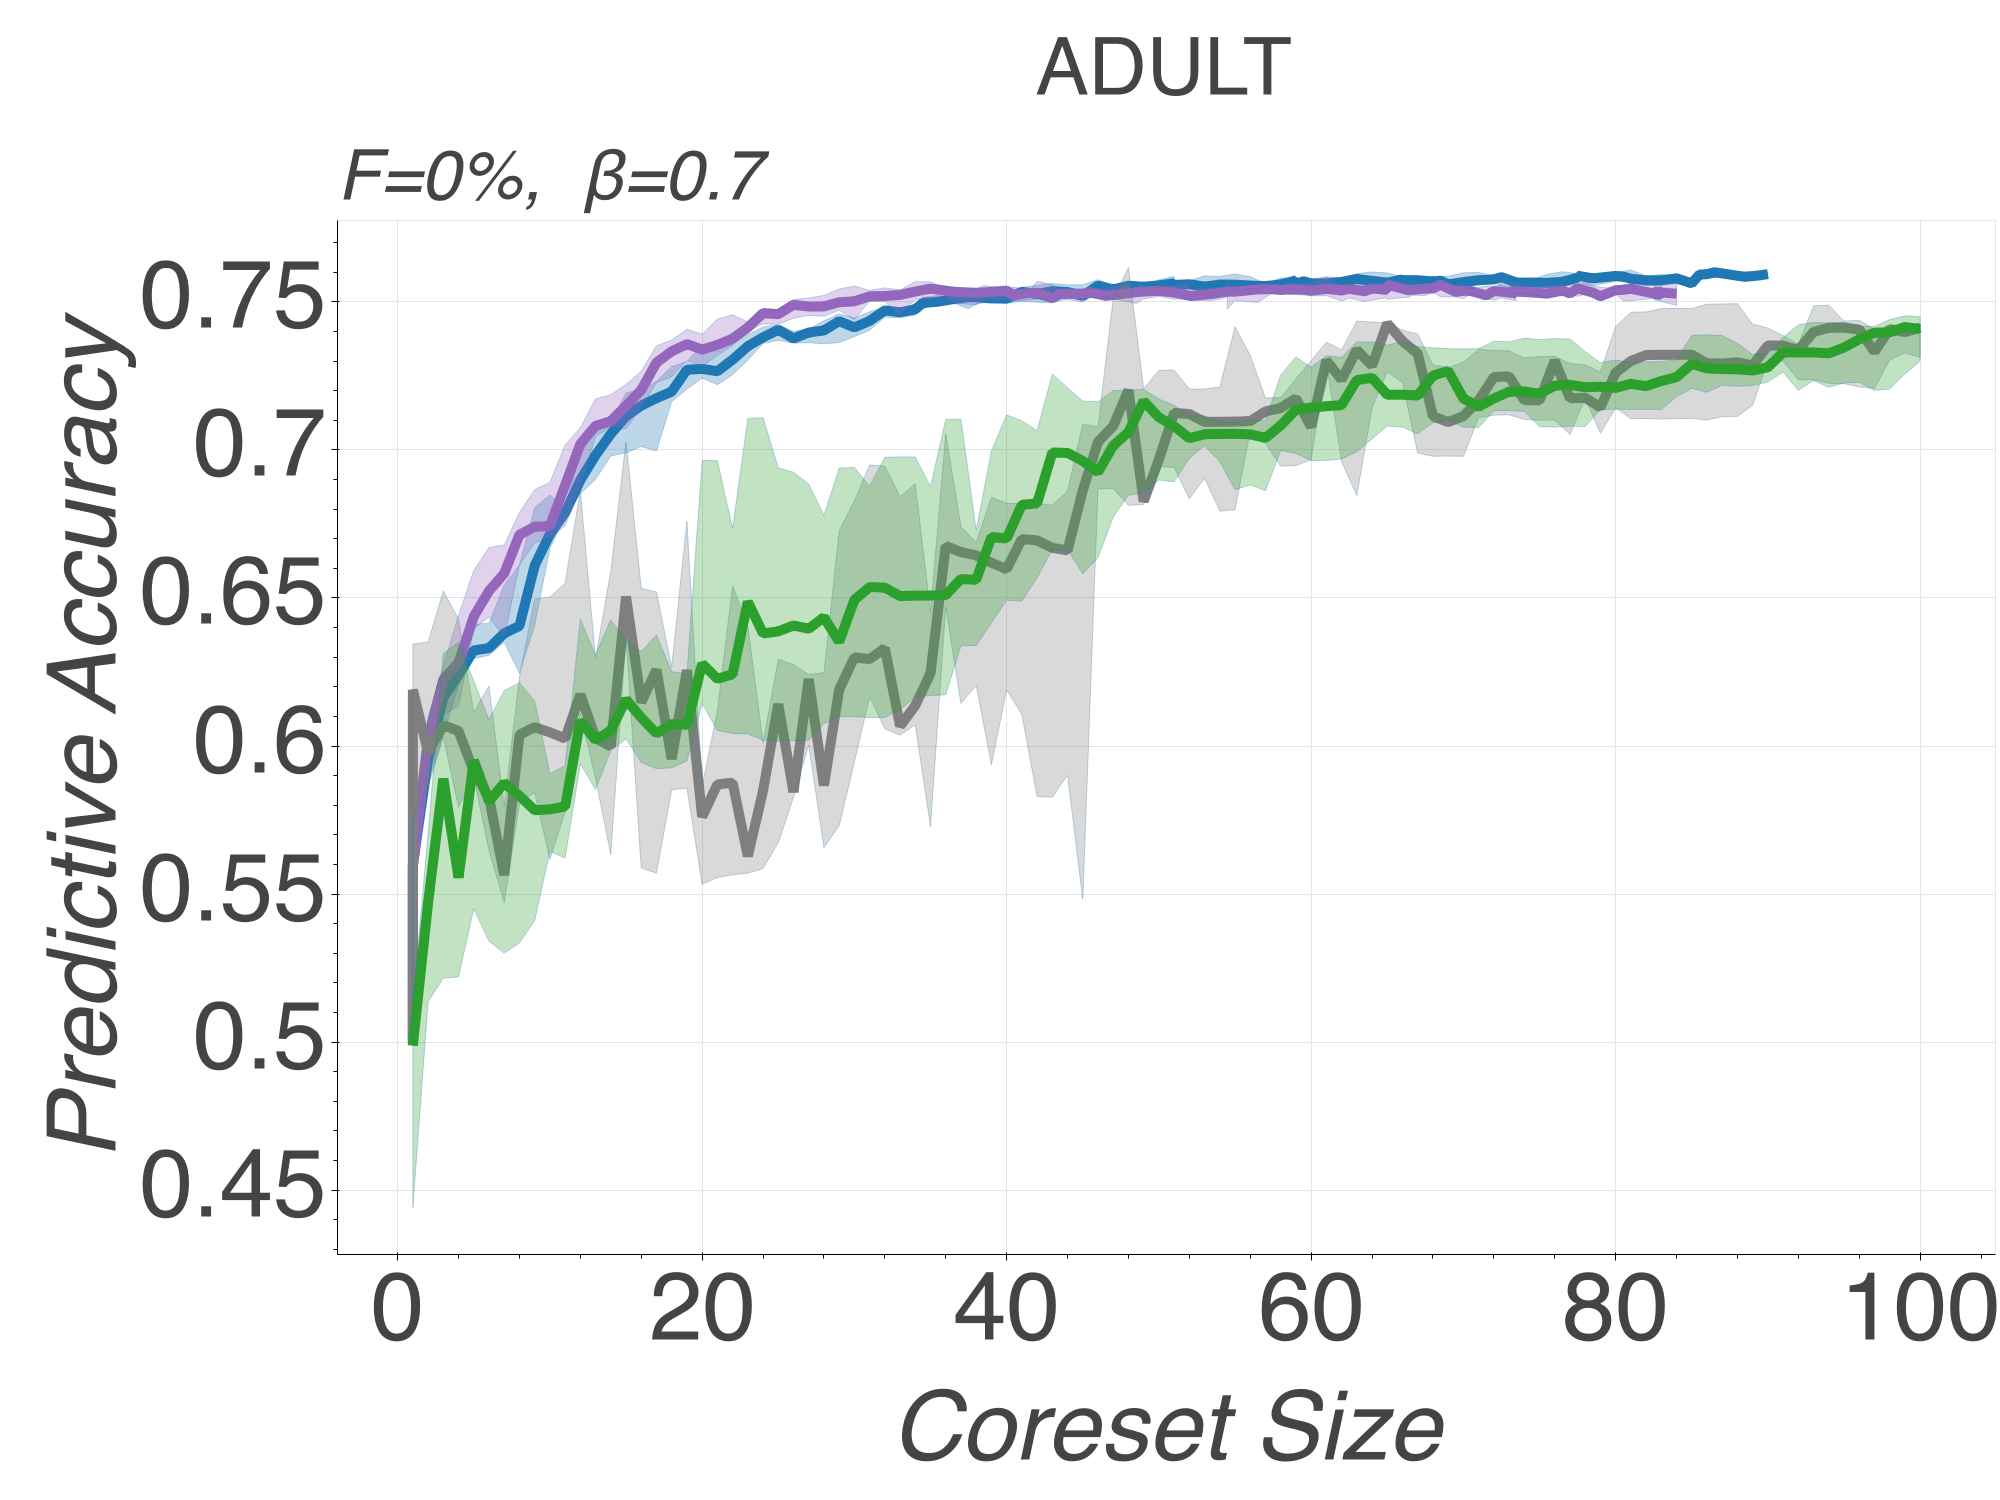
\includegraphics[width=.325\textwidth]{\MyPath/figs/adult07_10_0_False_False_ACCvssz.png}
		\centering
		\hfill
		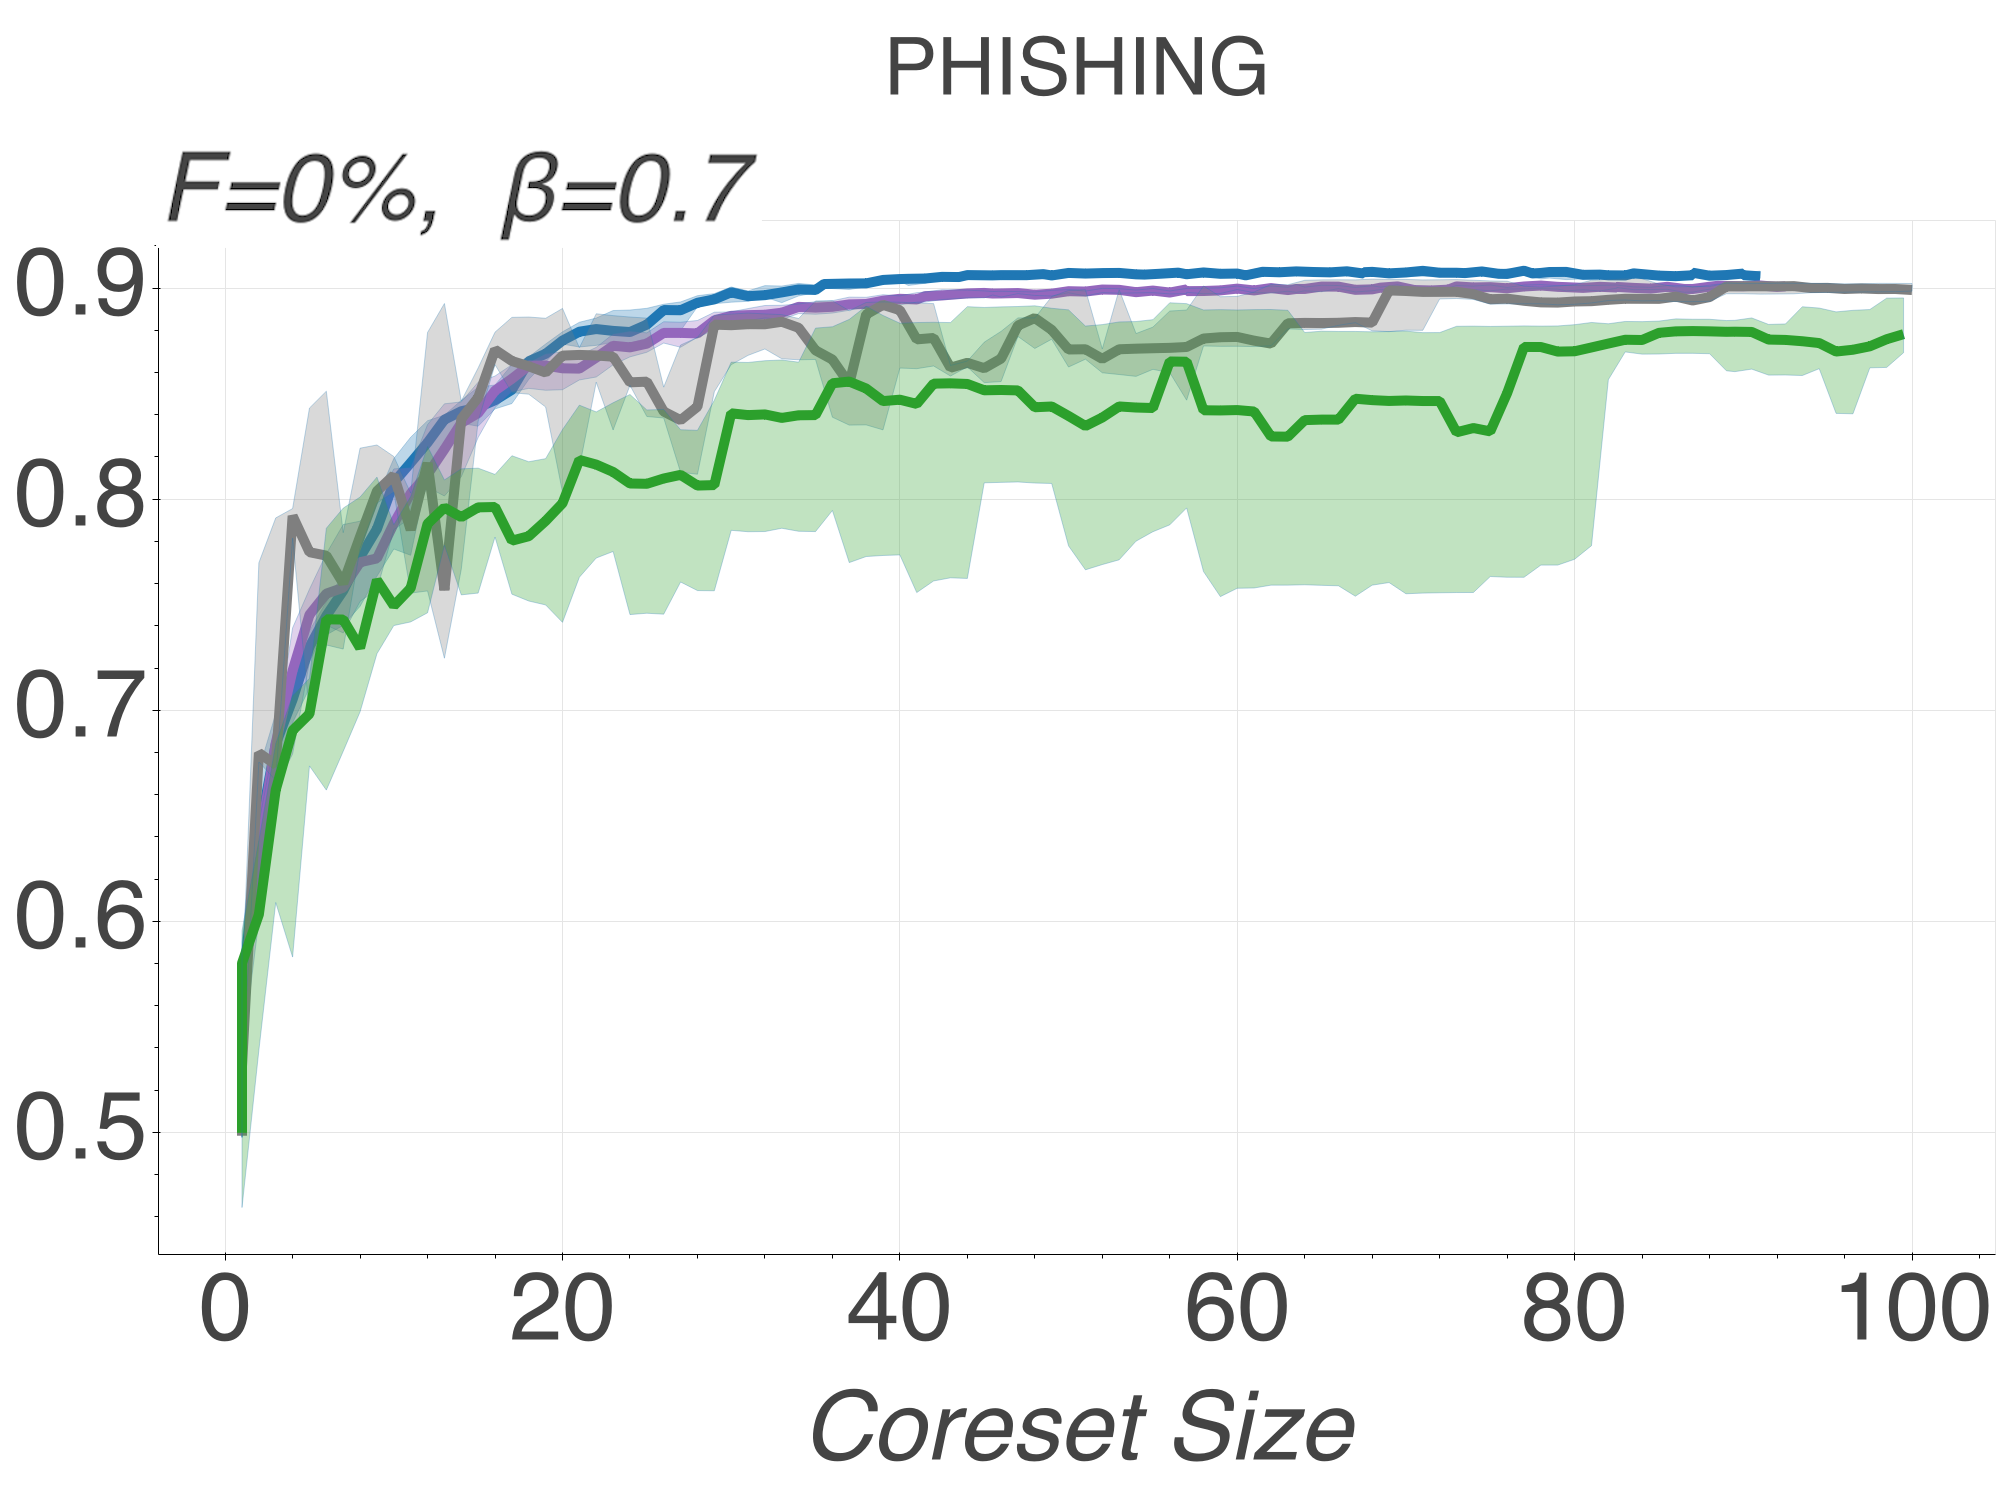
\includegraphics[width=.325\textwidth]{\MyPath/figs/phish07_10_0_False_False_ACCvssz.png}
		\centering
		\hfill
		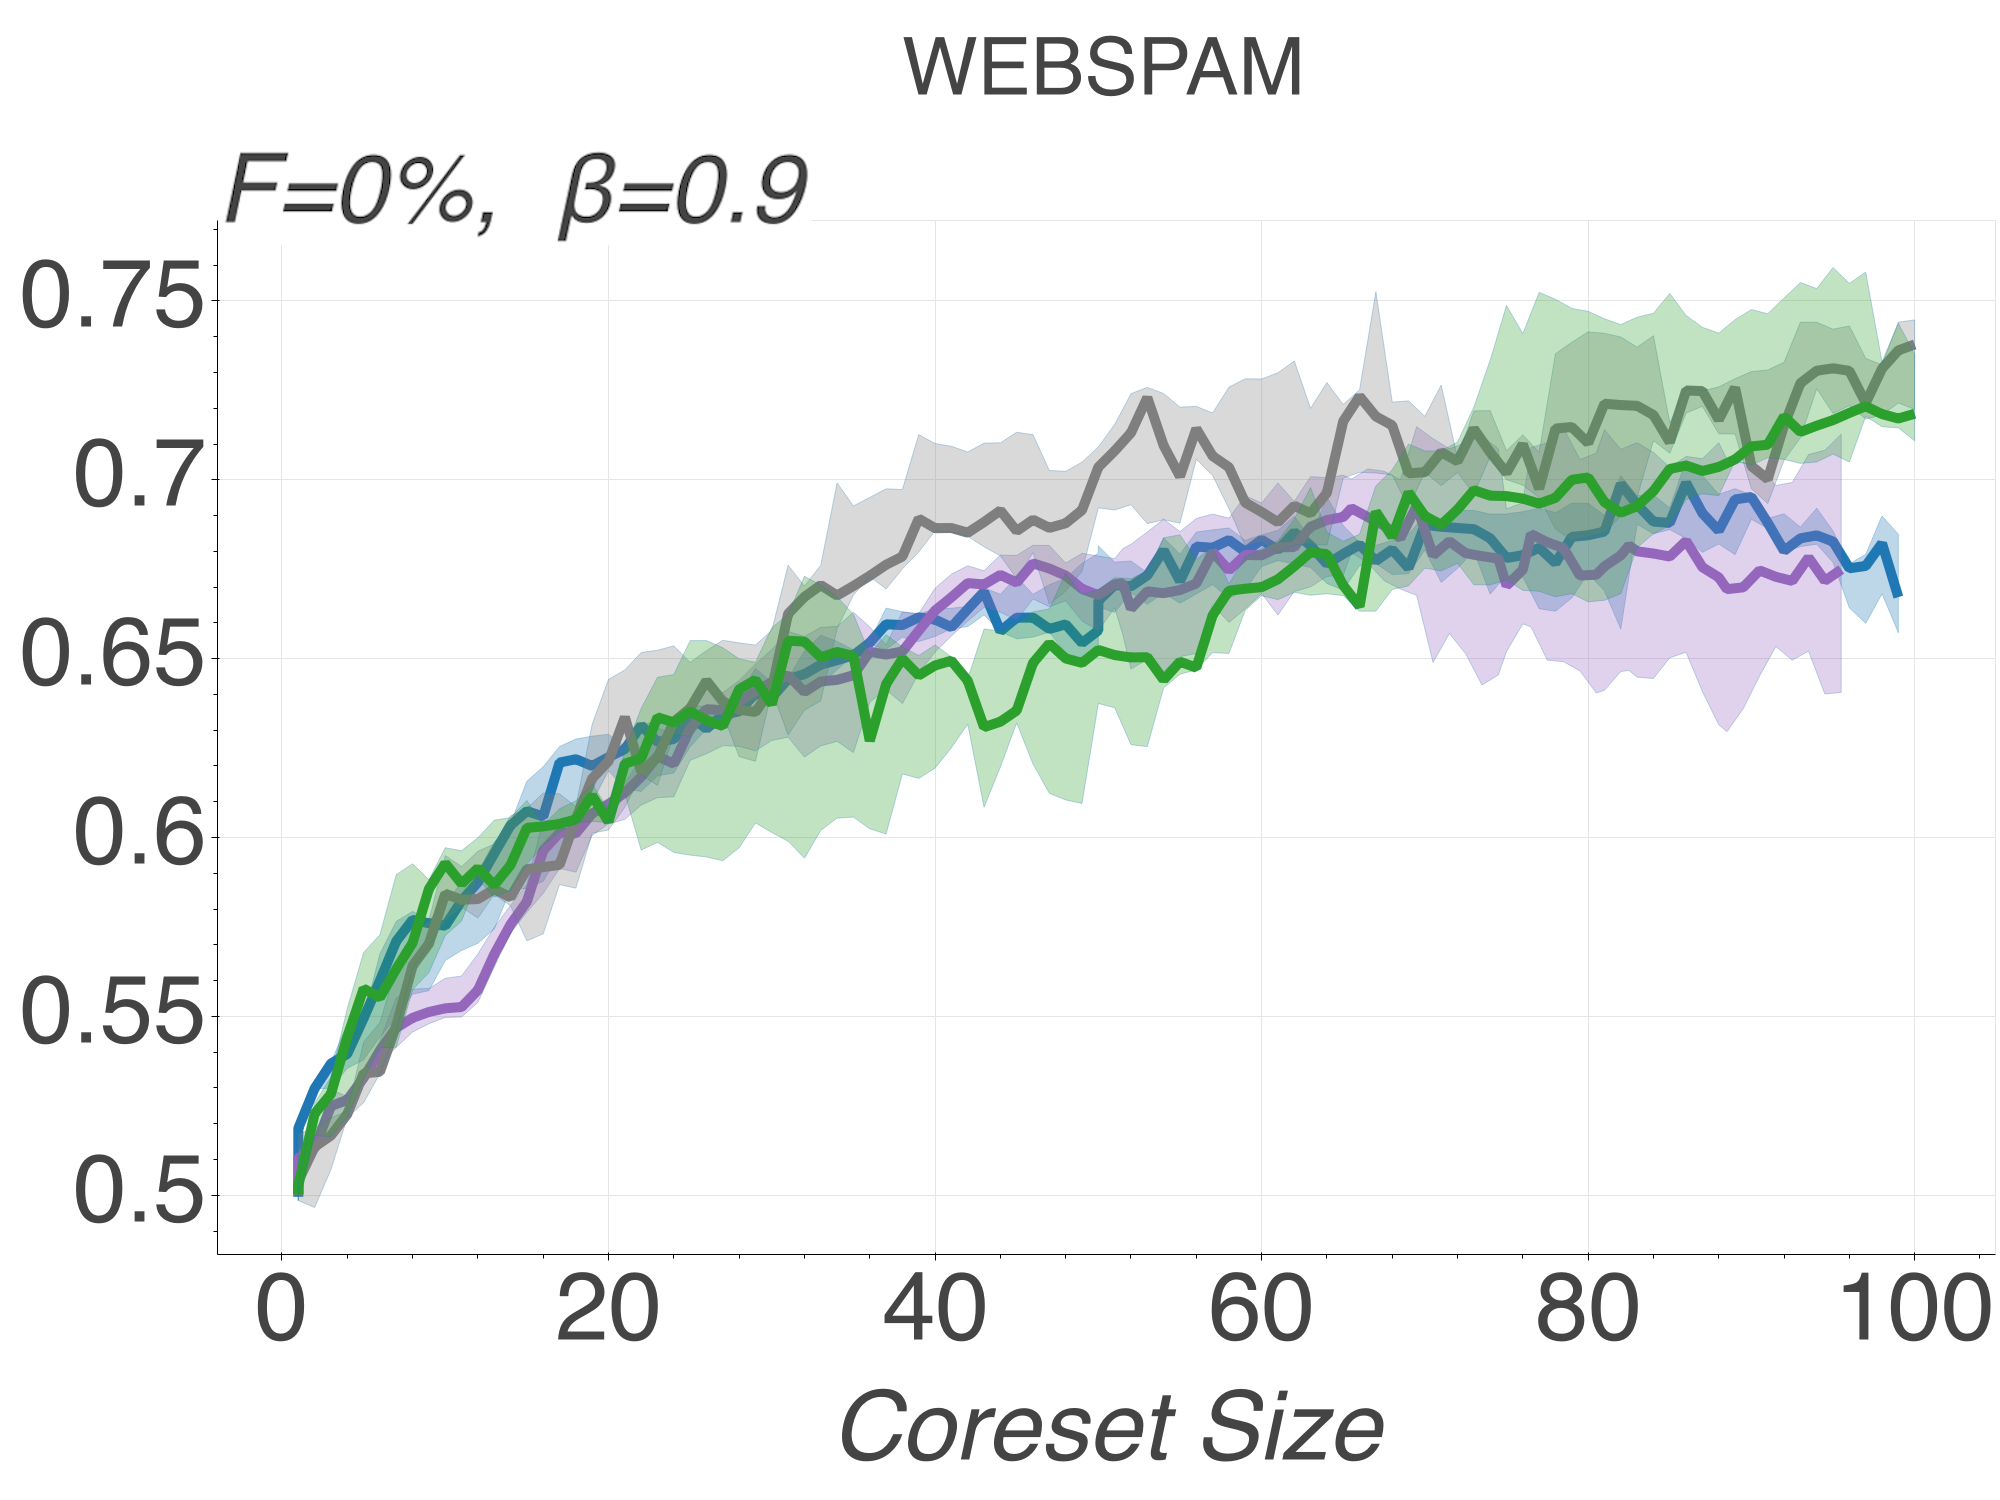
\includegraphics[width=.325\textwidth]{\MyPath/figs/webspam09_10_0_True_False_ACCvssz.png}
	\end{subfigure}	
	\centering
	\caption{Predictive accuracy vs coreset size for logistic regression experiments over $10$ trials on $3$ large-scale datasets. Solid lines display the median accuracy, with shaded areas showing $25\textsuperscript{th}$ and $75\textsuperscript{th}$ percentiles. Dataset corruption rate $F$, and $\beta$ value used in \bcores{} for each experiment are shown on the figures. The bottom row plots illustrate the achieved predictive performance under no contamination.}
	\label{fig:logreg_plot}
\end{figure}


\subsection{Neural Linear Regression on Noisy Data Batches}
\label{subsec:neur-linr-expt}

\begin{figure}[t!]
	\begin{subfigure}[b]{0.9\textwidth} 
		\centering
		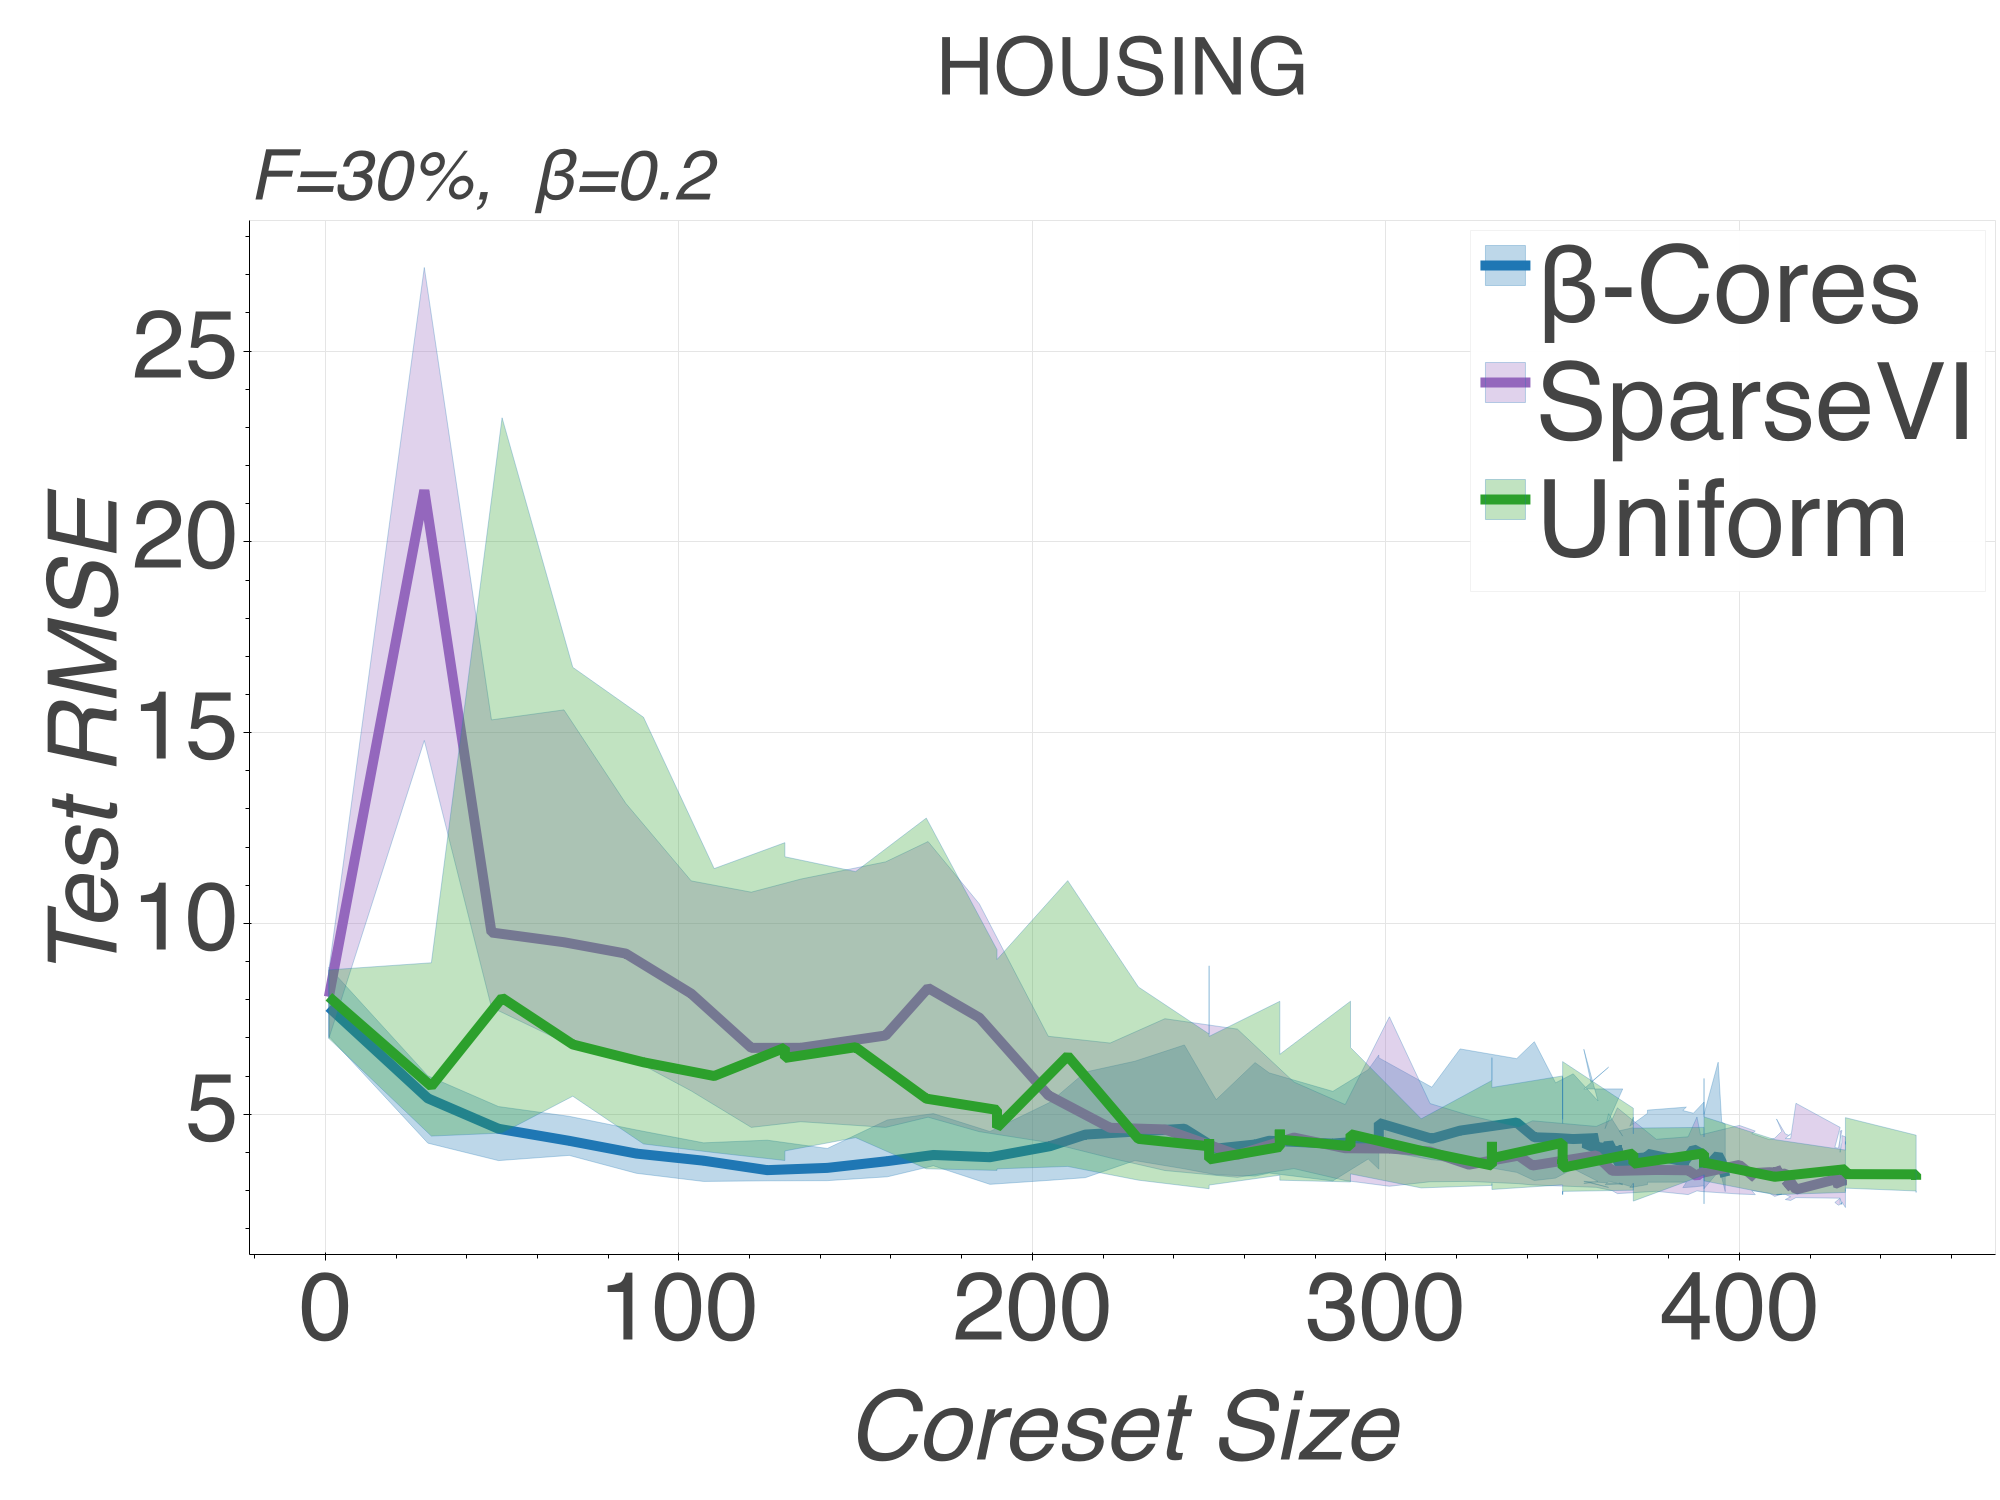
\includegraphics[width=.45\textwidth]{\MyPath/figs/boston02_01_30_RMSEvssz.png}
		\hfill
		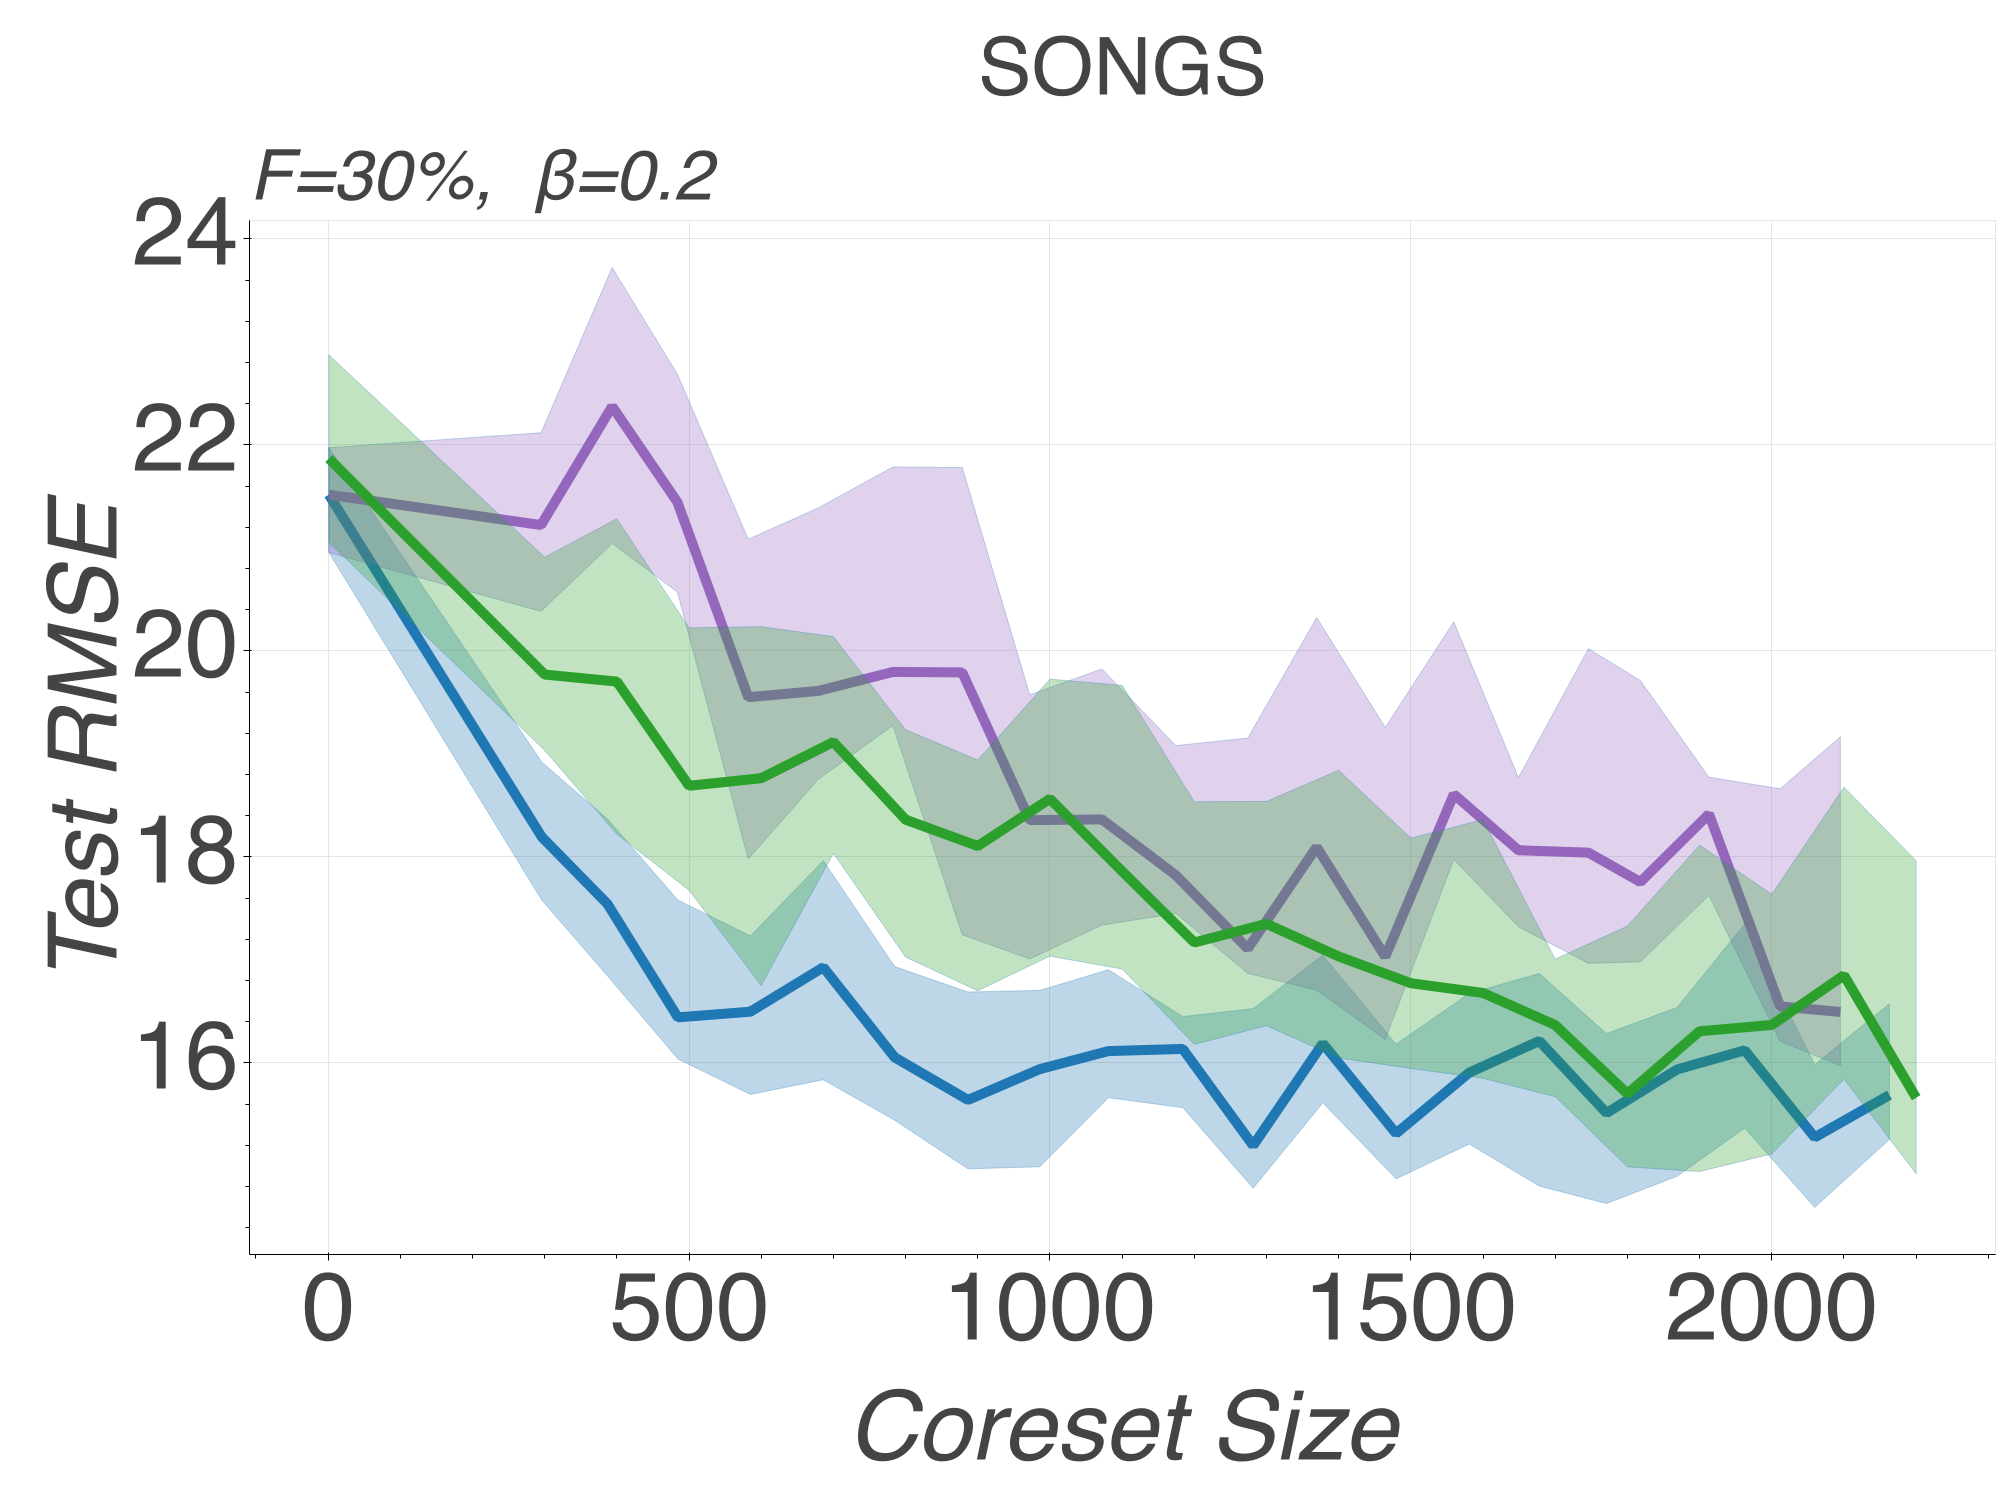
\includegraphics[width=.45\textwidth]{\MyPath/figs/year02_01_30_RMSEvssz.png}
		\centering
		\hfill
		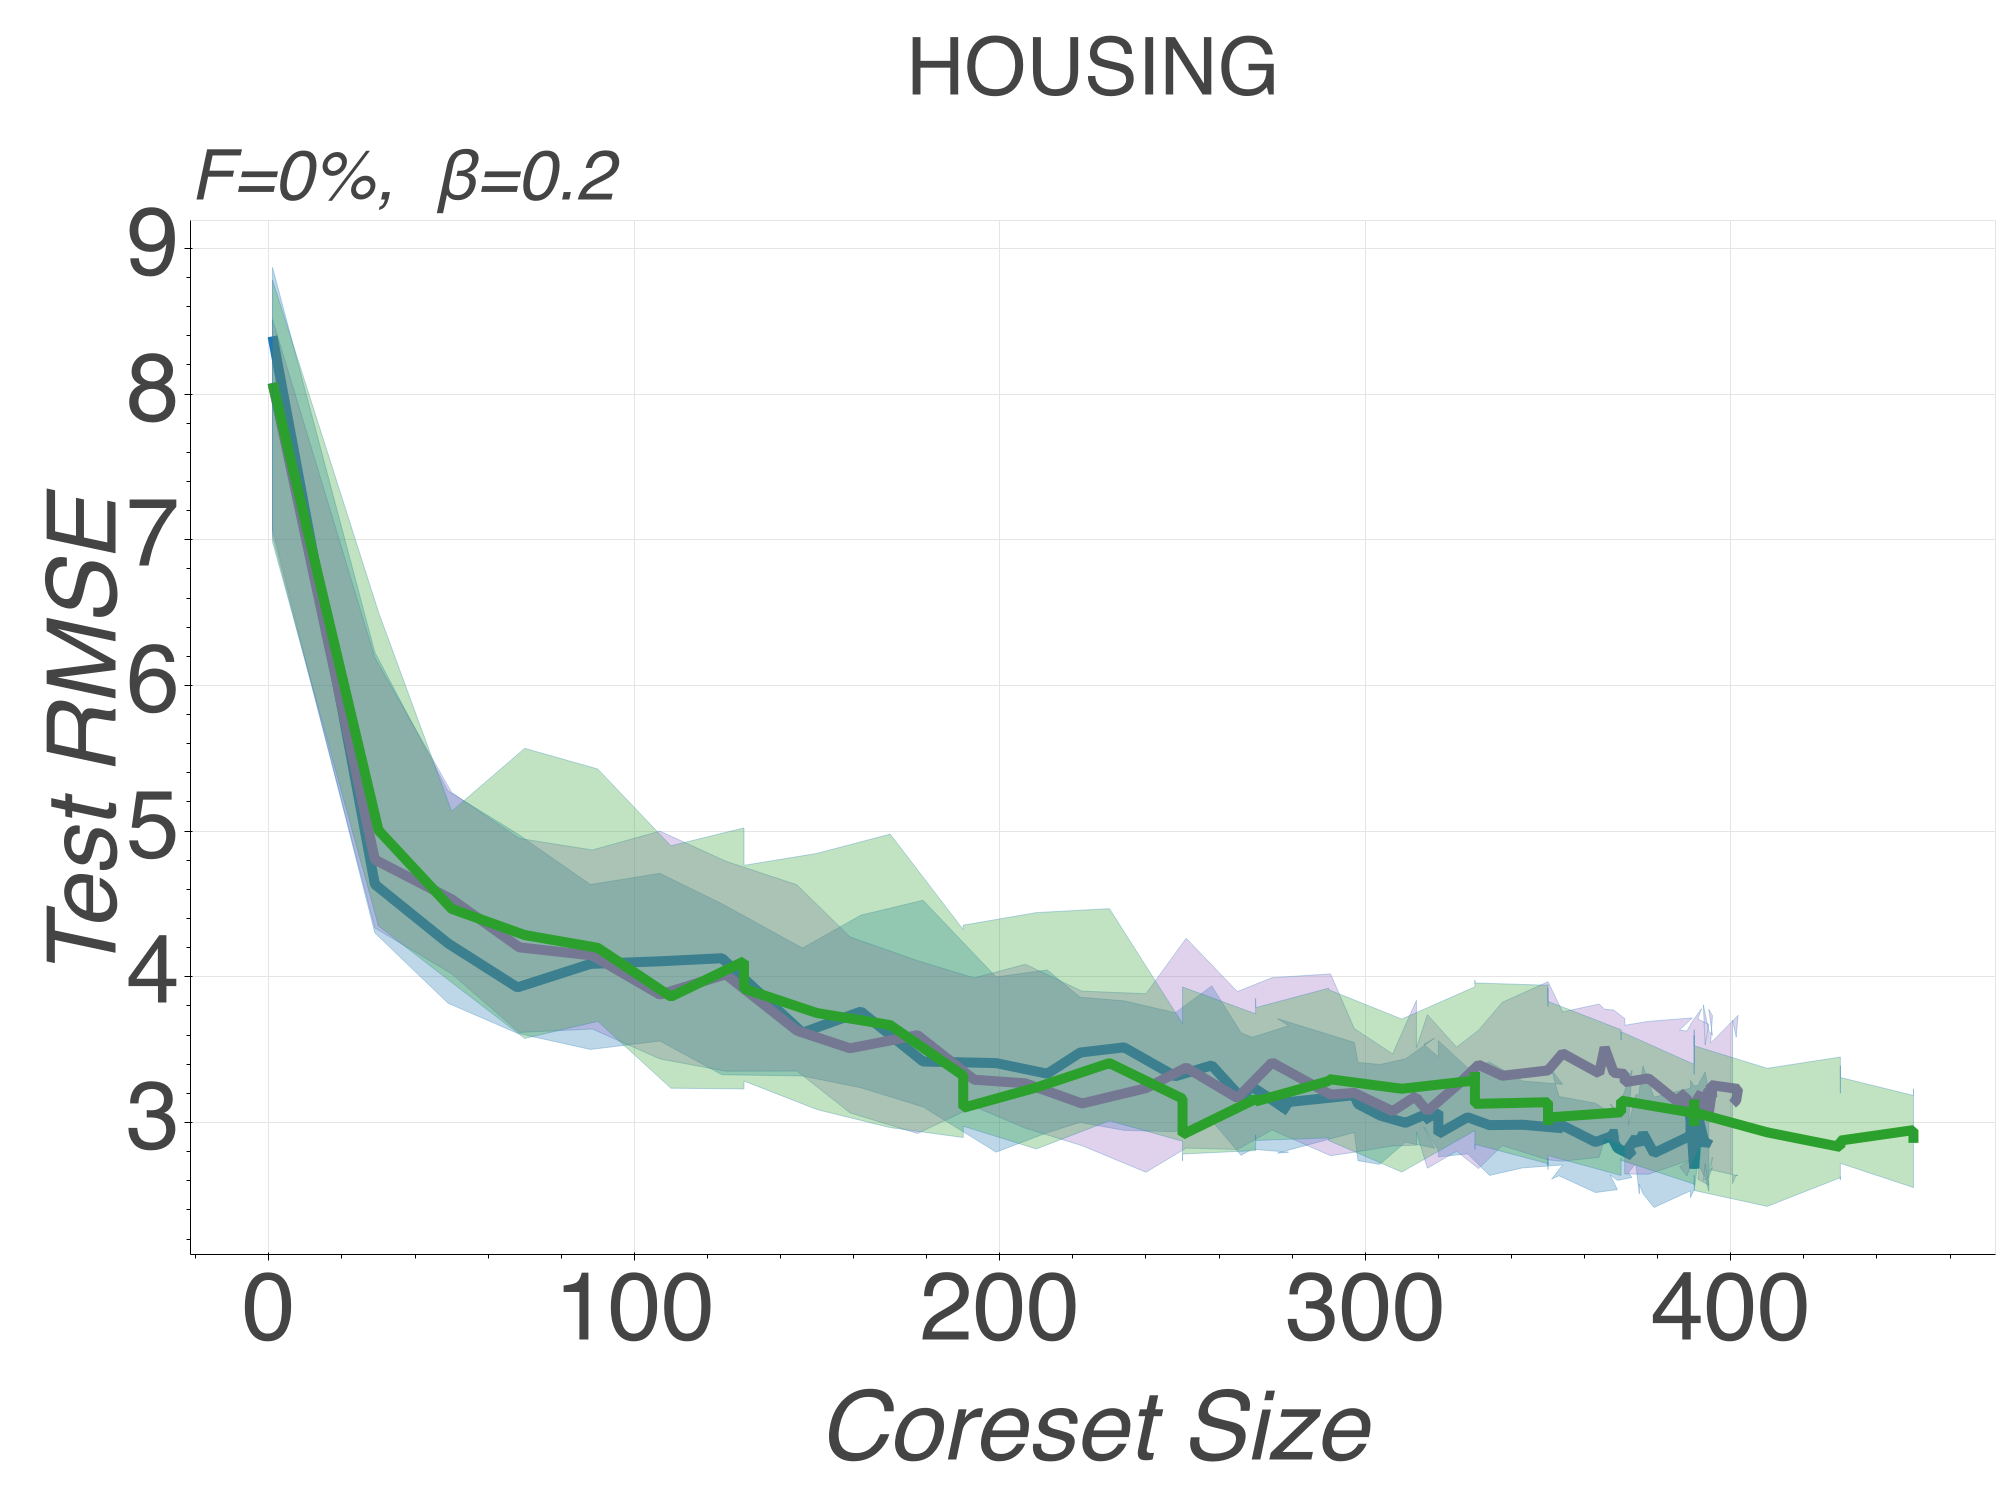
\includegraphics[width=.45\textwidth]{\MyPath/figs/boston02_01_0_RMSEvssz.png}
		\centering
		\hfill
		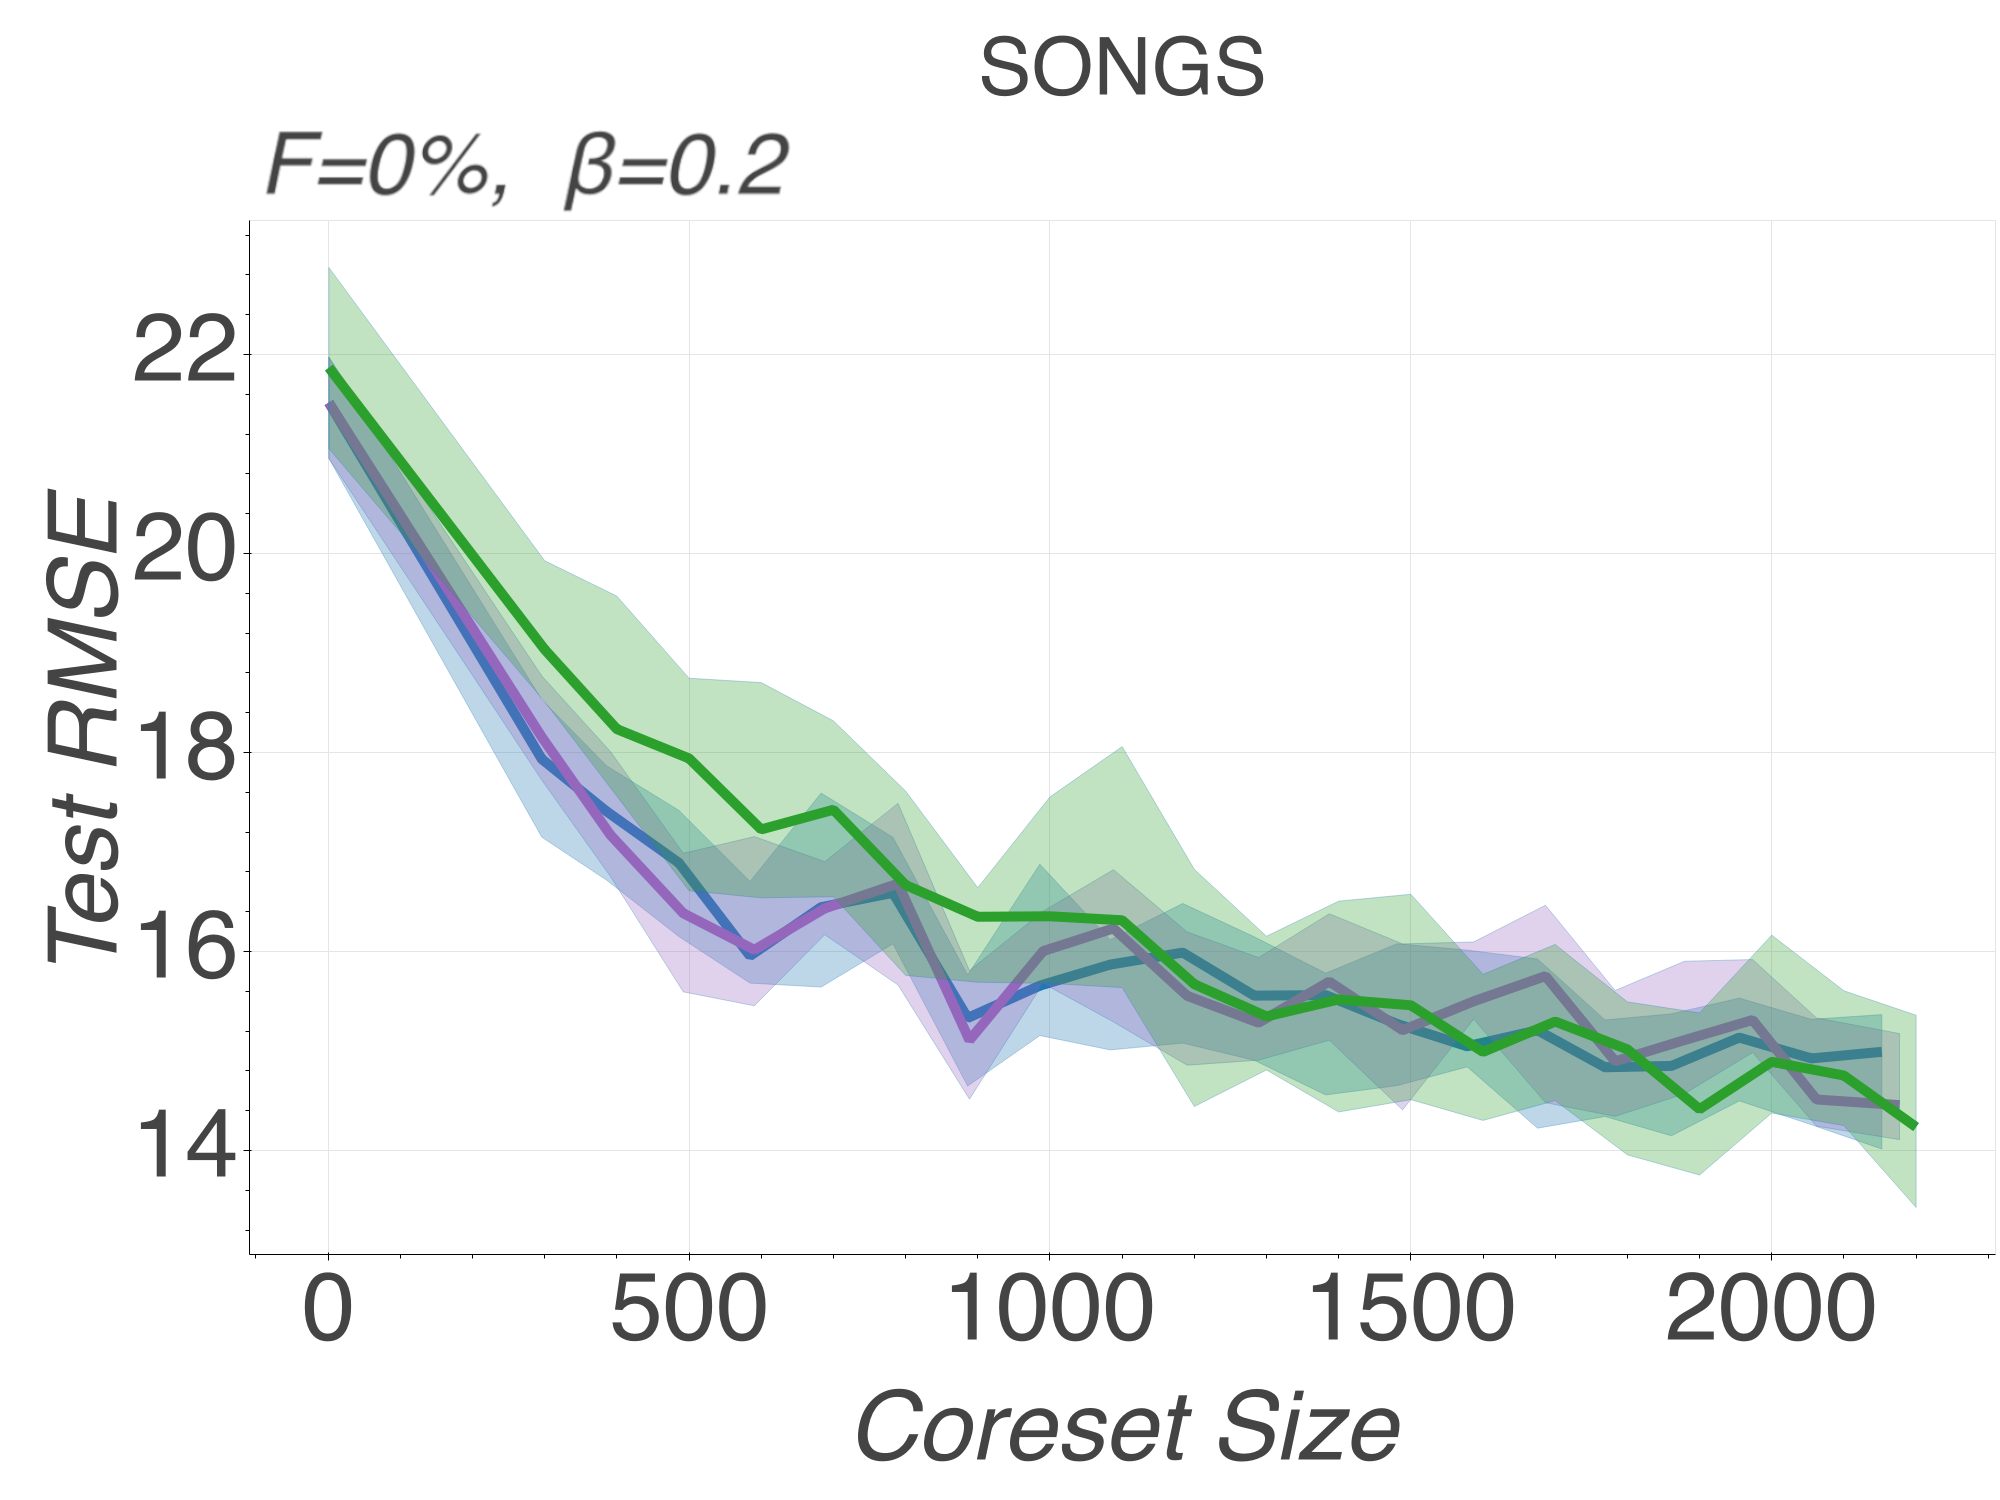
\includegraphics[width=.45\textwidth]{\MyPath/figs/year02_01_0_RMSEvssz.png}
	\end{subfigure}	
	\centering
	\caption{Test RMSE vs coreset size for neural linear regression experiments averaged over 30 trials. Solid lines display the median RMSE, with shaded areas showing $25\textsuperscript{th}$ and $75\textsuperscript{th}$ percentiles. Dataset corruption rate $F$, and $\beta$ value used in \bcores{} for each experiment are shown on the figures. The bottom row plots illustrate the achieved predictive performance under no contamination.}
	\label{fig:neural_plot}
\end{figure}

Here we use the coresets extension for batch summarization to efficiently train a neural linear model on selected data minibatches. Neural linear models perform Bayesian linear regression on the representation of the last layer of a deterministic neural network feature extractor~\cite{snoek15,riquelme18,pinsler19}.
The corresponding statistical model is as follows
\[
%&z(\cdot) \dist \distNorm(\mu_0, \sigma_0^2 I), \\
%\quad 
&\left(y_n\right)_{n=1}^{N} = \theta^T z(x_n) + \eps_n,
\quad
\left(\eps_n\right)_{n=1}^{N} \dist \distNorm(0, \sigma^2).
\label{eq:neurlinr-stat-model}
\]
The neural network is trained to learn an adaptive basis $z(\cdot)$ from $N$ datapoint pairs $(x_n,y_n) \in \reals^{d} \times \reals$, which we then use to regress $ \left(y_n\right)_{n=1}^{N} $ on $ \left(z(x_n)\right)_{n=1}^{N} $, and yield uncertainty aware estimates of $\theta$. More details on the model-specific formulae entering coresets construction are provided in~\cref{sec:neurlinr-lik}. Input and output related outliers are simulated as in~\cref{subsec:logreg-expt}, while here, for the output related outliers, $y_n$  gets replaced by Gaussian noise. Corruption occurs over a percentage $F\%$ of the total number of minibatches of the dataset, while the remaining minibatches are left uncontaminated. Each poisoned minibatch gets $70\%$ of its points \mbox{substituted by outliers}.

We evaluate \bcores, \sparsevi{} and random sampling on two benchmark regression datasets~(detailed in~\cref{sec:data-details}). All coresets are initialized to a small batch of datapoints sampled uniformly at random from the dataset inliers. Over incremental construction, we interleave each minibatch selection and weights optimization step of the coreset with a training round for the neural network, constrained on the current coreset datapoints. Each such training round consists of $10^3$ minibatch gradient descent steps using the AdaGrad optimizer~\cite{duchi11}.
Our neural architecture is comprised of two fully connected hidden layers, batch normalization and ReLU activation functions. The values of coreset size at initialization, batch size added per coreset iteration, and units at each neural network hidden layer are set respectively to 20, 10 and 30 for the~\textsc{Housing}, and 200, 100 and 100 for the~\textsc{Songs} dataset.


\cref{fig:neural_plot}~(bottom row) shows that \bcores{} are competitive with the baselines in the absence of data corruption, achieving similar predictive performance over the entire range of tested coreset sizes. Under data poisoning~(top row), \bcores{} is the only method that offers monotonic decrease of test RMSE for increasing summary size from the beginning of the experiment. On the other hand, baselines present unreliable predictive performance for small coreset sizes: random sampling and \sparsevi{} are both prone to including corrupted data batches, whose misguiding information gets expressed on the flexible representations learnt by the neural network, requiring a larger summary size to reach the RMSE of \bcores.





\subsection{Efficient Data Acquisition from Subpopulations for Budgeted Inference}
\label{sec:active-selection}


We consider the scenario where a machine learning service provider aims to fit a binary classification model to observations coming from multiple subpopulations of data contributors. The provider aims to maximize the predictive accuracy of the model, while adhering to a budget on the total number of subpopulations from which data can be used over inference. Budgeted inference can be motivated by several practical requirements: First, restricting the total number of datapoints used over learning to a smaller informative subset aids scalability---which is the primary motivation for coresets. Moreover, taking decisions at the subpopulations level regarding which groups of datapoints are useful for the task, without the need to inspect datapoints individually, reduces the privacy loss incurred over the data selection stage, and can be integrated in machine learning pipelines that follow formal hierarchical privacy schemes. Finally, subpopulations valuation can guide costly experimental procedures, via inducing knowledge regarding which group combinations are most beneficial in summarizing the entire population of interest~\citep{pinsler19, vahidian20}, and hence should be prioritised over data collection.

In this study we use a subset of more than $60K$ datapoints from the \textsc{HospitalReadmissions} dataset (for further details see \cref{sec:data-details}). Using combinations of age, race and gender information of data contributors, we form a total of $165$ subpopulations within the training dataset. Data contamination is simulated identically to the experiment of \cref{subsec:logreg-expt}, while now we also consider the case of varying levels of contamination across the subpopulations. In particular, we form groups of roughly equal size where $0\%, 10\%$ and $20\%$ of the datapoints get replaced by outliers---this results in getting a dataset with approximately $10\%$ of its full set of datapoints corresponding to outliers.


\begin{figure}[t!]
	\begin{subfigure}[b]{0.9\textwidth} 
		\centering
		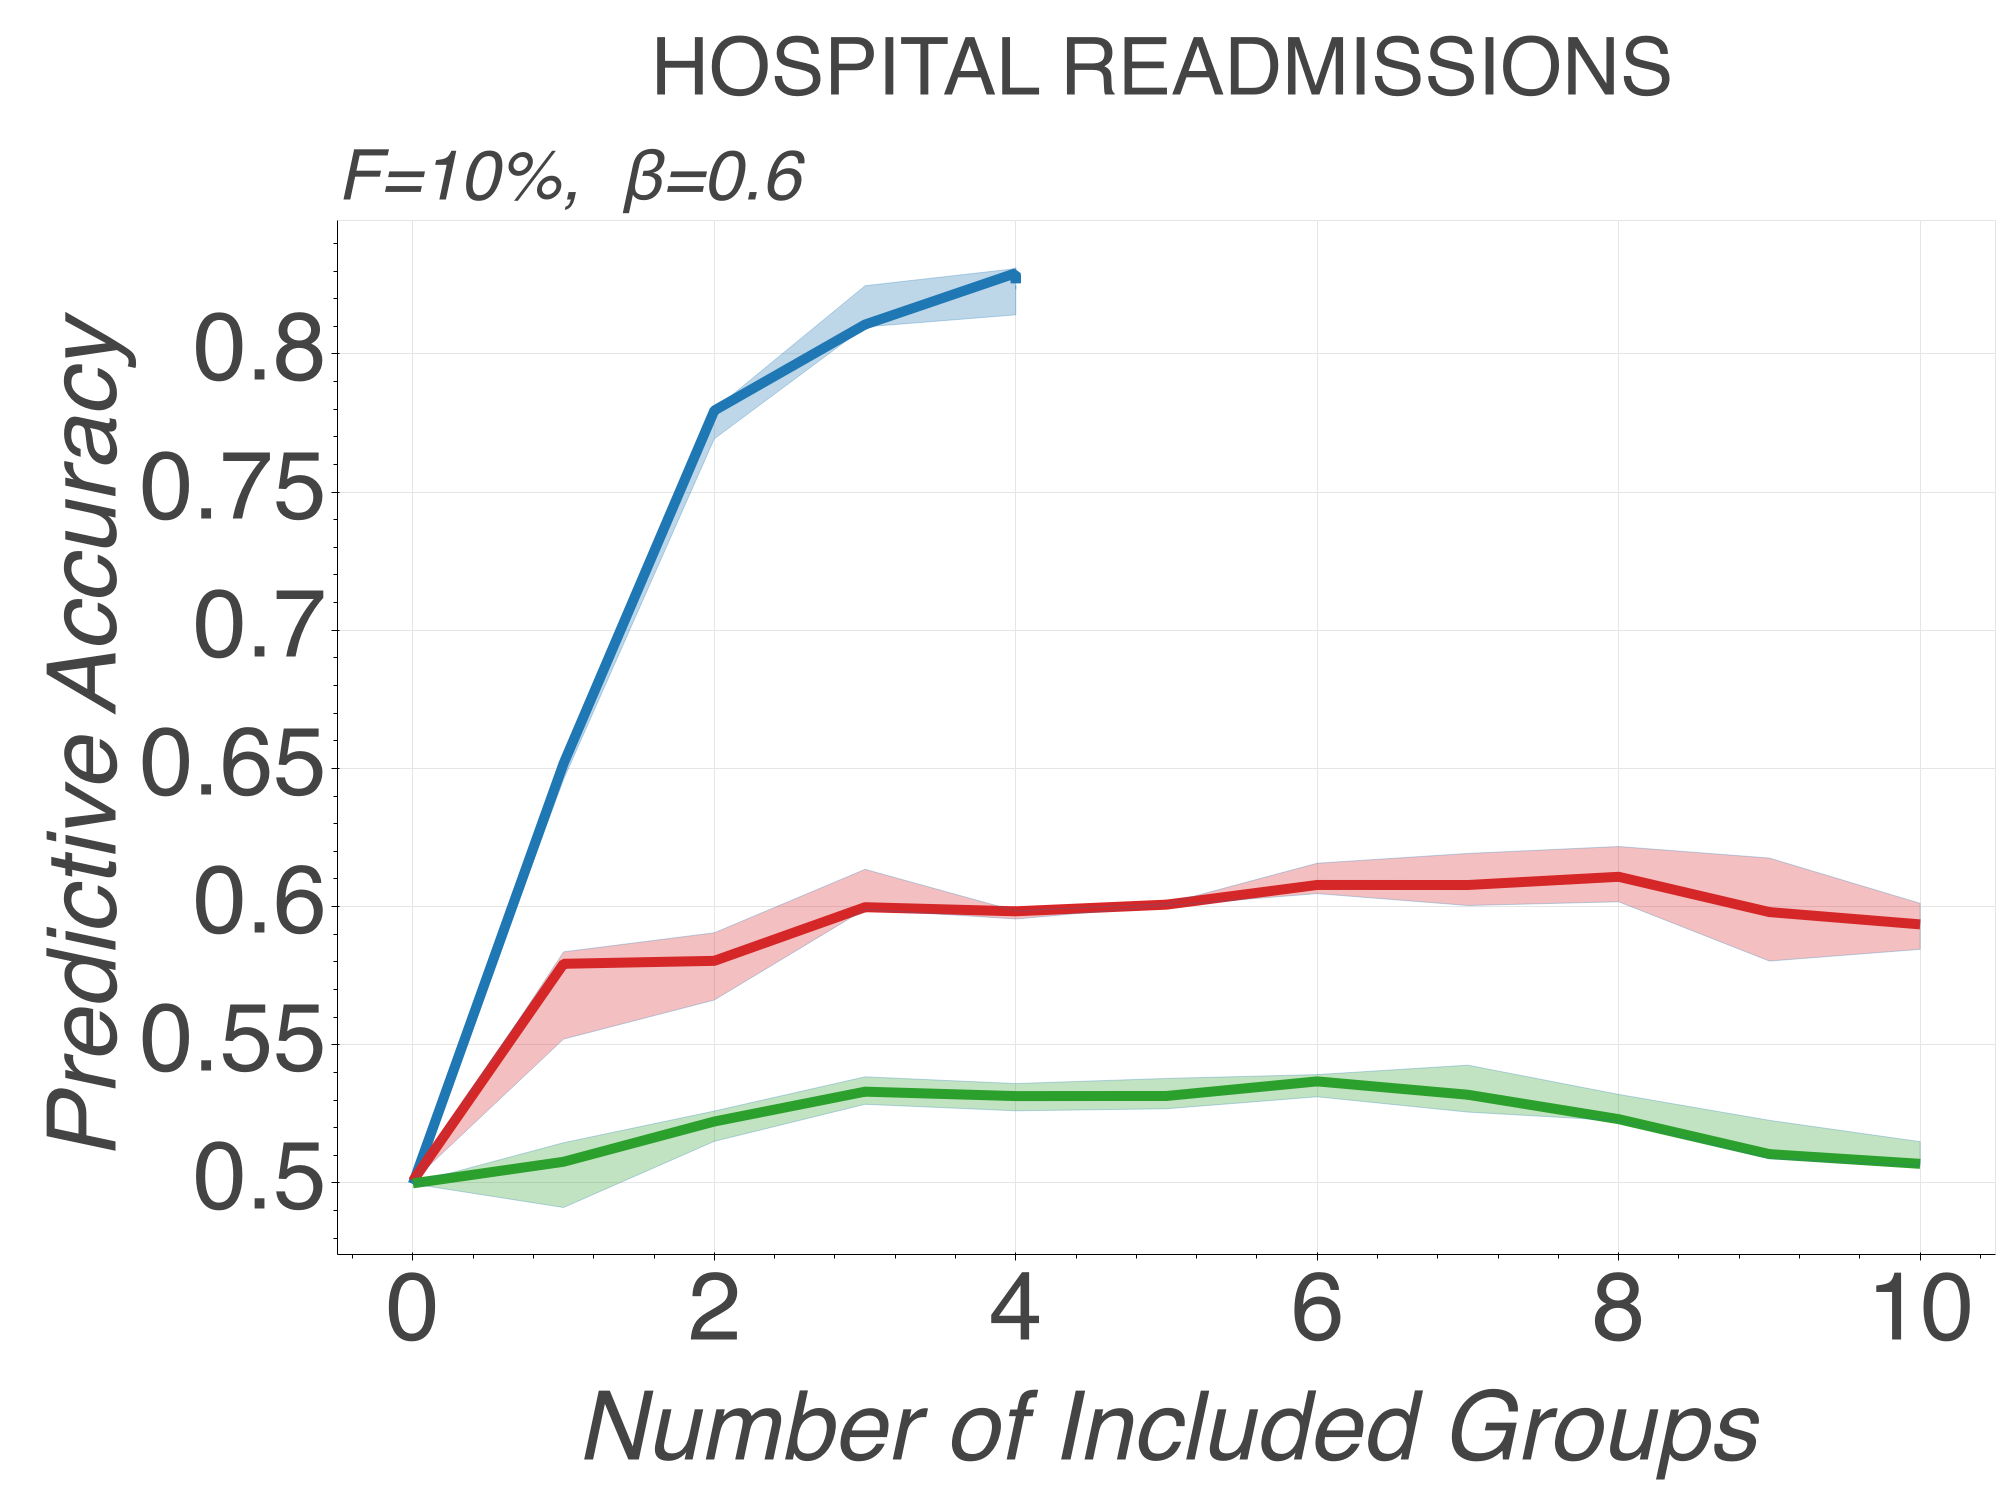
\includegraphics[width=.45\textwidth]{\MyPath/figs/group_diabetes06_10_01_False_ACCvsit.png}
		\hfill
		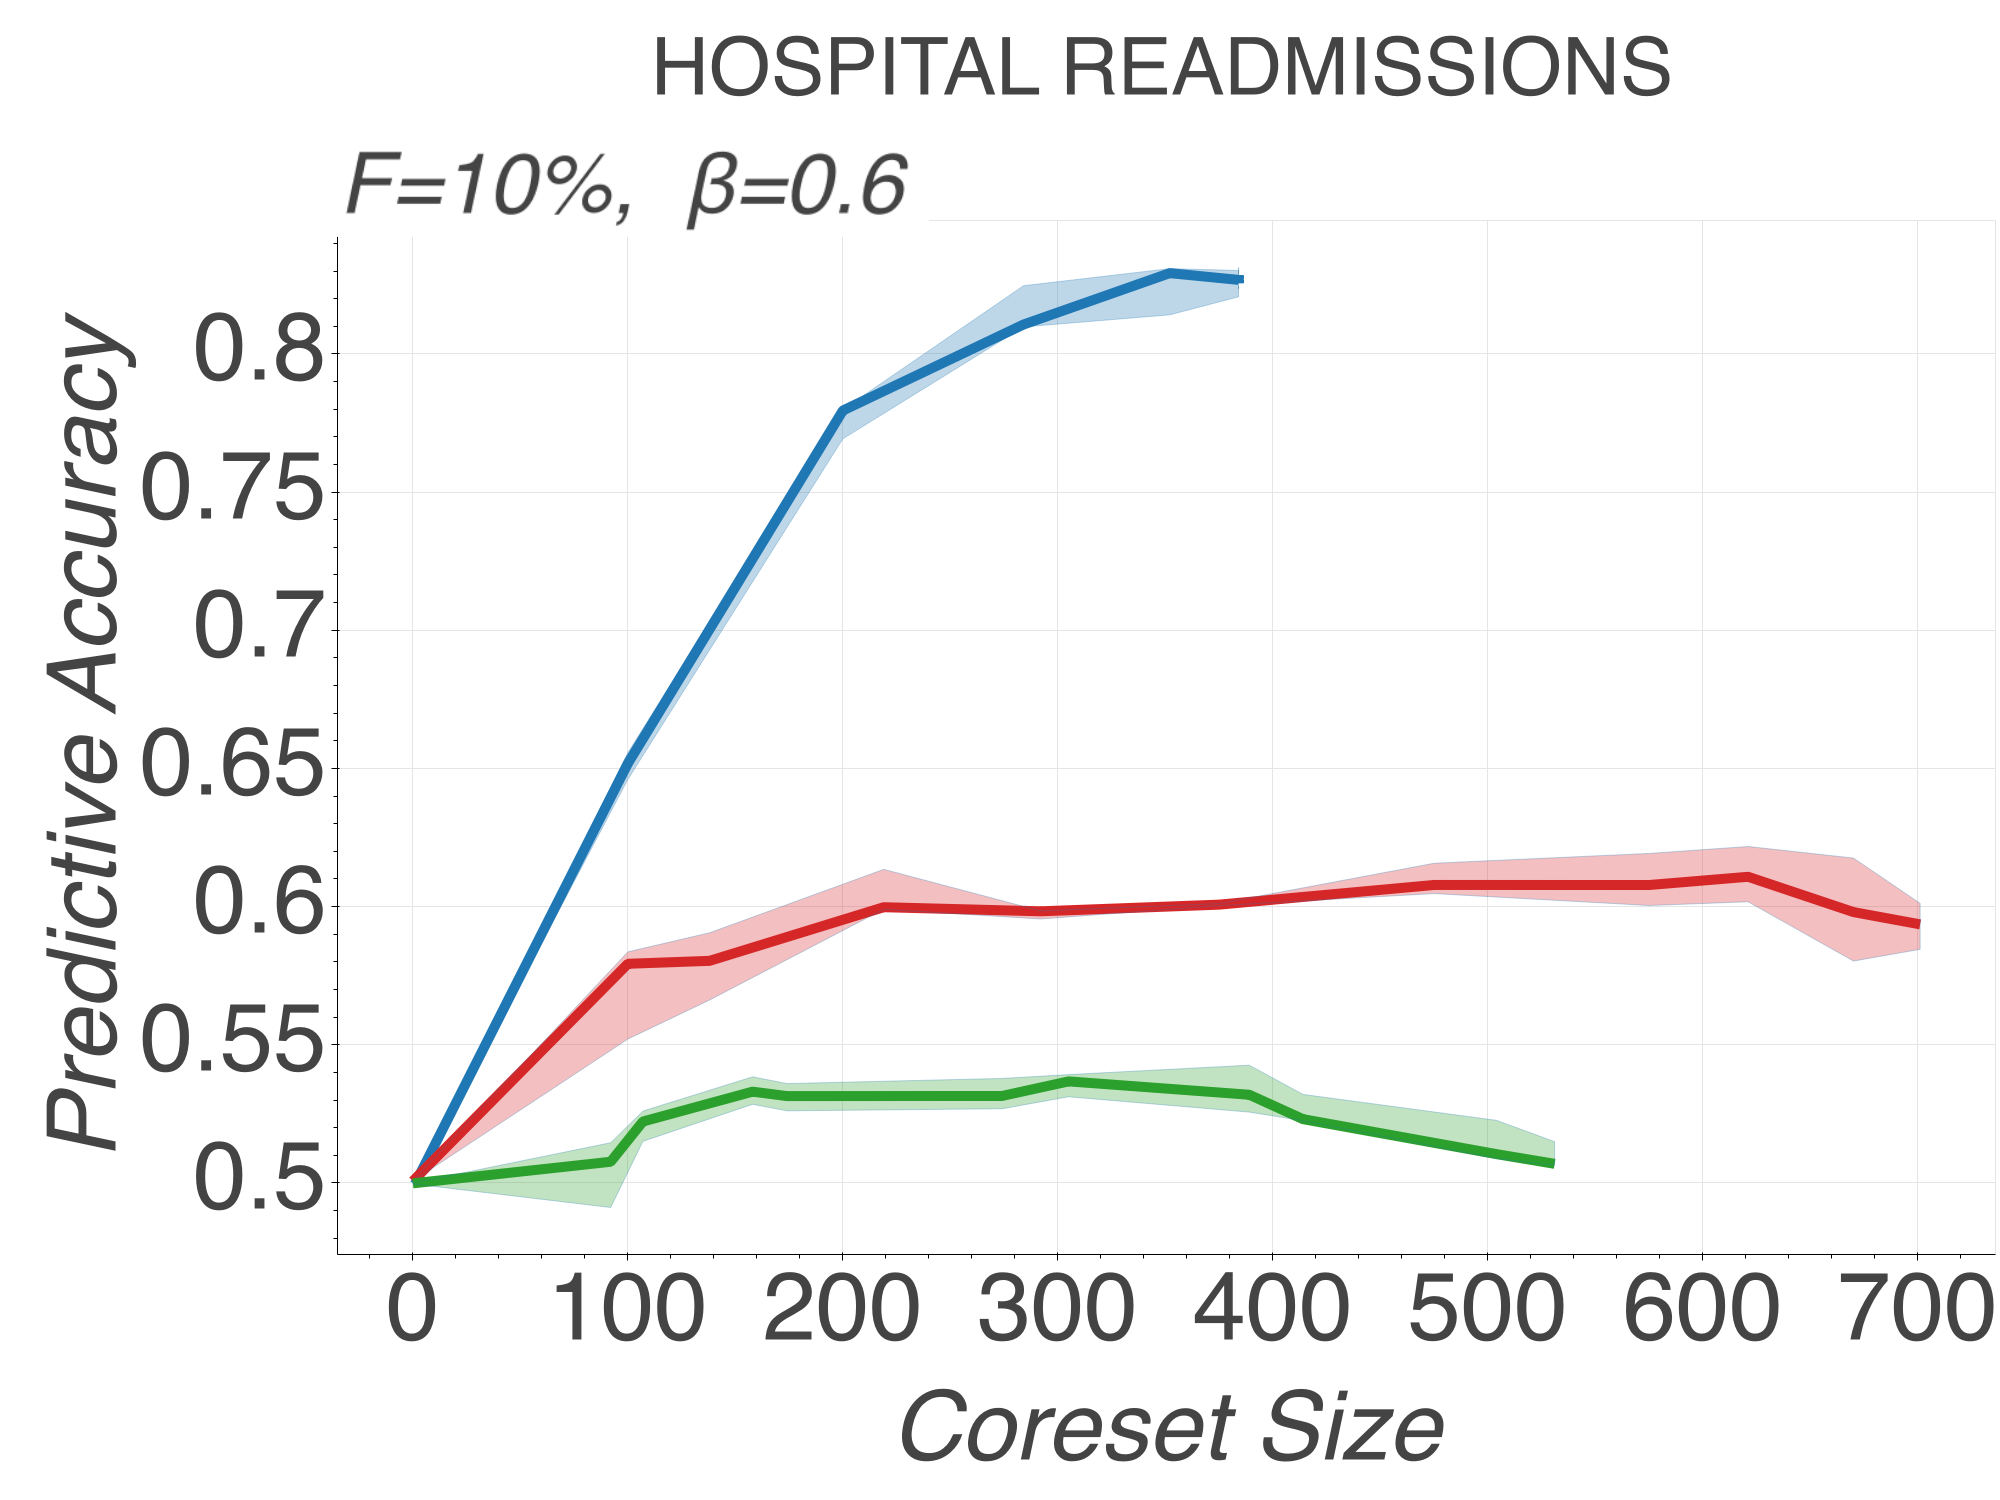
\includegraphics[width=.45\textwidth]{\MyPath/figs/group_diabetes06_10_01_False_ACCvssz.png}
		\centering
		\hfill
		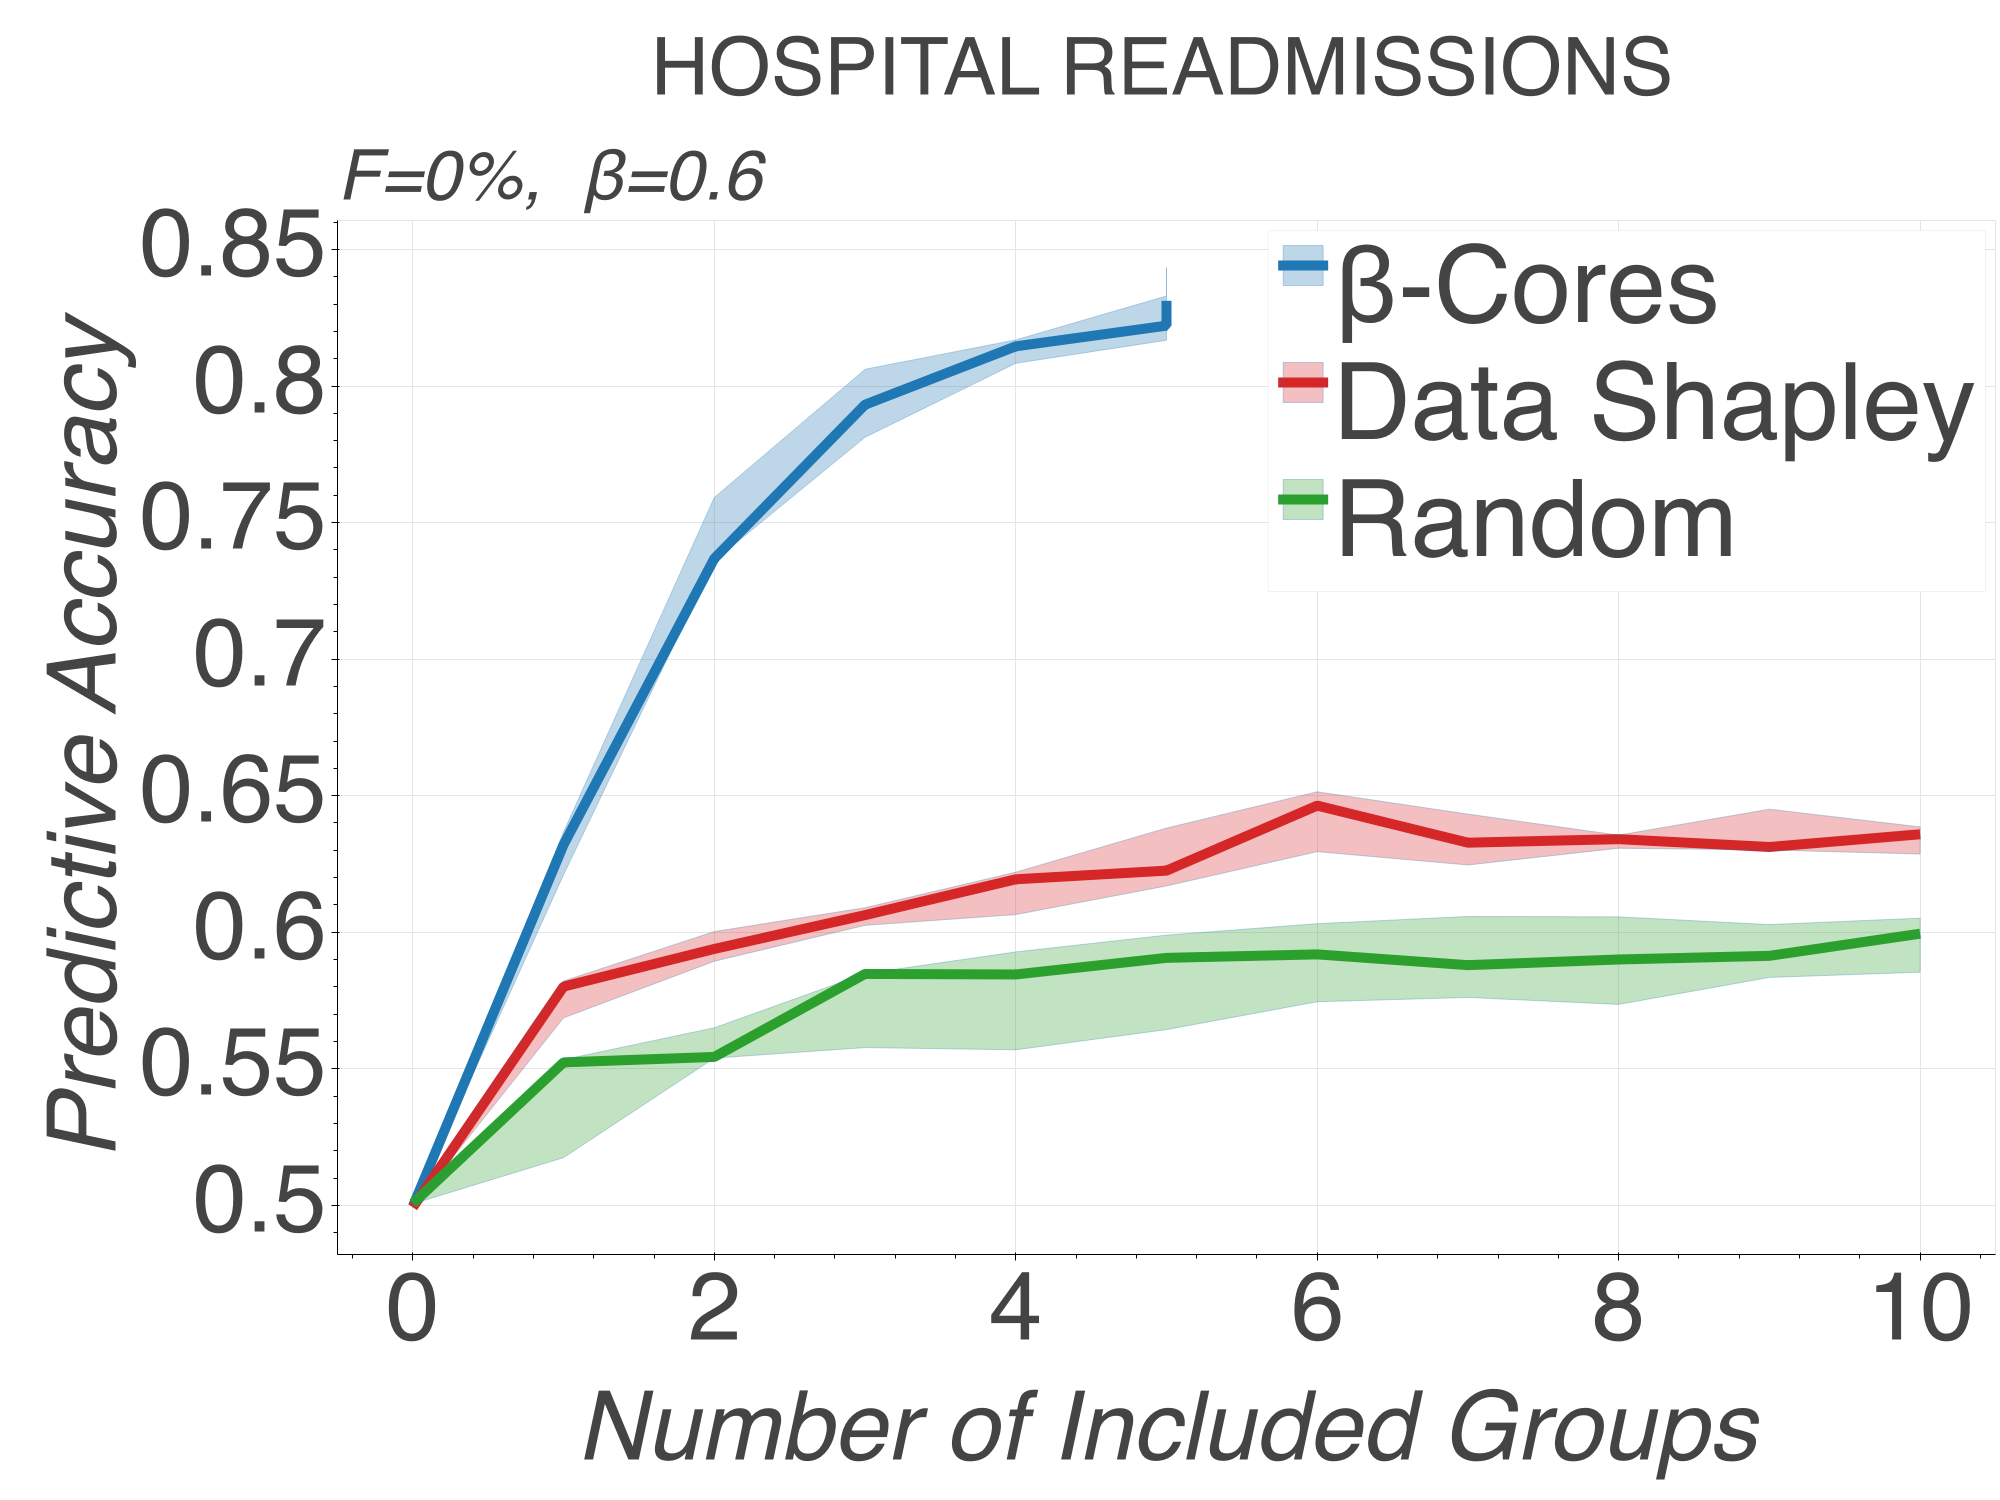
\includegraphics[width=.45\textwidth]{\MyPath/figs/group_diabetes06_10_0_False_ACCvsit.png}
		\centering
		\hfill
		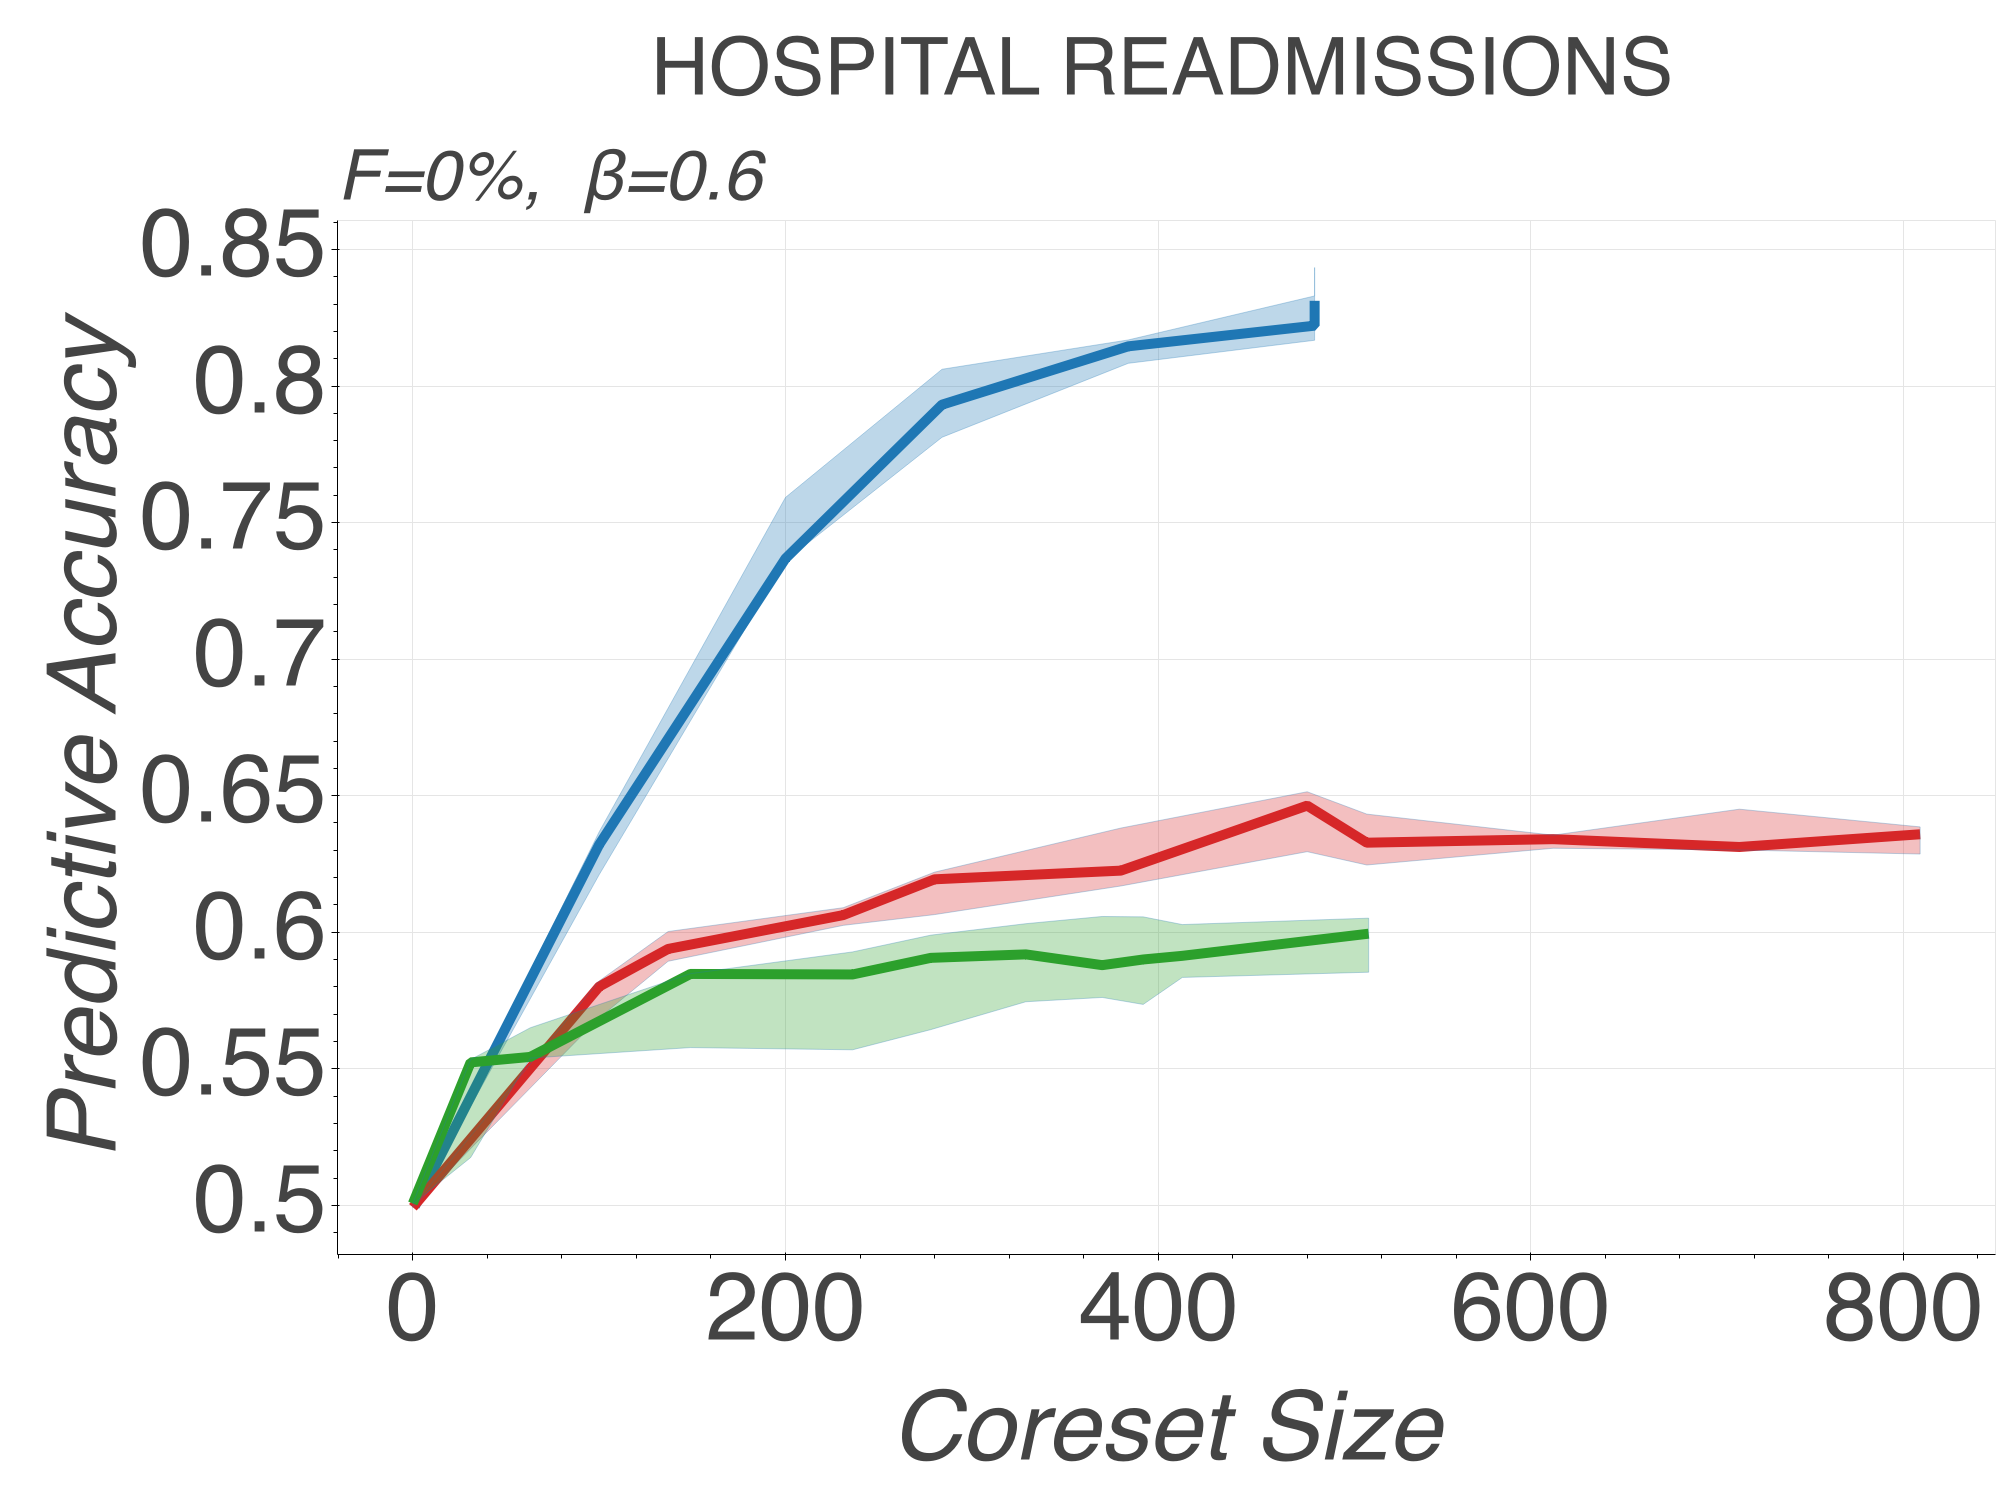
\includegraphics[width=.45\textwidth]{\MyPath/figs/group_diabetes06_10_0_False_ACCvssz.png}
	\end{subfigure}	
	\centering
	\caption{Predictive accuracy against number of groups~(left) and number of datapoints~(right) selected for inference. Compared group selection shemes are \bcores{}, selection according to Shapley values based ranking, and random selection. The experiment is repeated over $5$ trials, on a contaminated dataset containing a $10\%$ of crafted outliers distributed non-uniformly across groups~(top row), and a clean dataset~(bottom row).}
	\label{fig:group_plot}
\end{figure}


We evaluate the predictive accuracy achieved by doing inference on the data subset obtained after running $10$ iterations of the \bcores{} extension for groups (which gives a maximum of $10$ selected groups). We compare against (\emph{i}) a \emph{random sampler}, and (\emph{ii}) a baseline which ranks all groups according to their \emph{Shapley value} and selects the groups with the highest values. Shapley value is a concept originating in cooperative game theory~\citep{shapley53}, which has recently found applications in data valuation and outliers detection~\cite{ghorbani19}. In the context of our experiment, it quantifies what is the marginal contribution of each group to the predictive accuracy of the model at all possible group coalitions that can be formed. As this quantity is notoriously expensive to be computed in large datasets, we use a Monte Carlo estimator which samples $5K$ possible permutations of groups and for each permutation it computes marginals for coalitions formed by the first $20$ groups.\footnote{The latter truncation is supported by the observation that marginal contributions to the predictive accuracy are diminishing as the dataset size increases.}

\begin{figure}[t!]
	\begin{subfigure}[b]{.8\textwidth} 
		\centering
		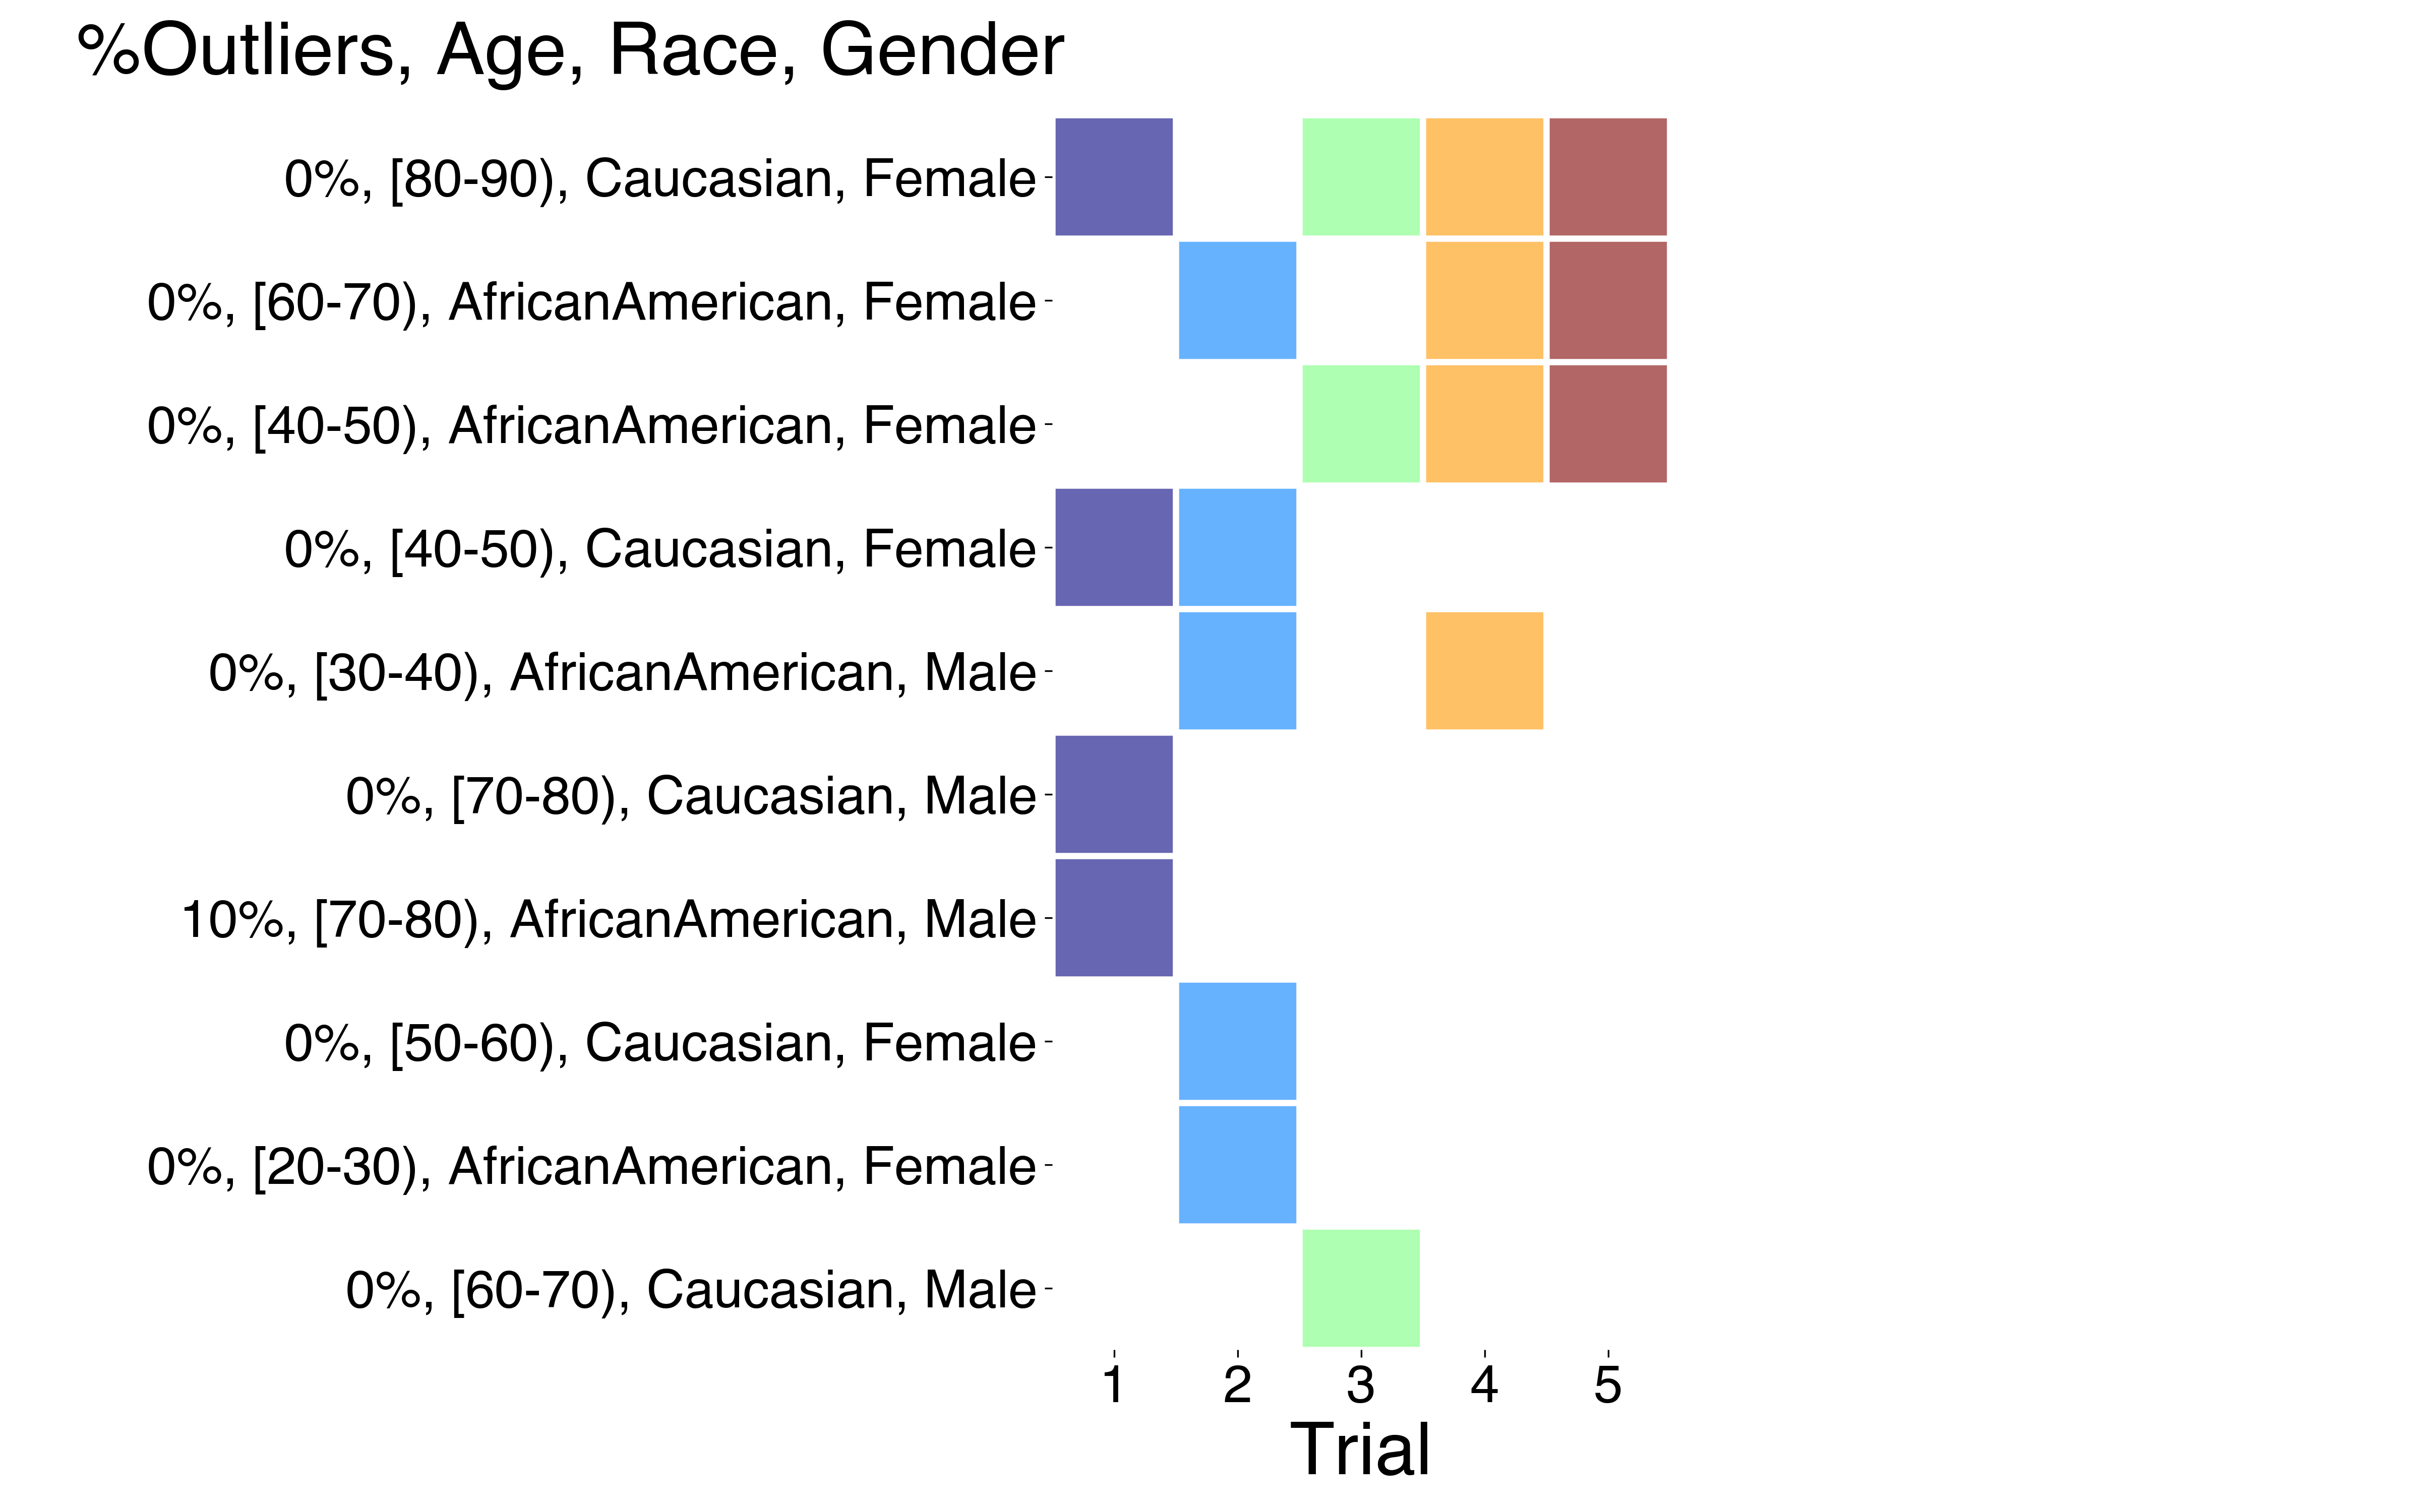
\includegraphics[width=.9\textwidth]{\MyPath/figs/selected_groups.png}
	\end{subfigure}	
	\centering
	\caption{Attributes of selected groups after running $10$ iterations of \bcores{} with $\beta=0.6$ on the contaminated \textsc{HospitalReadmissions} dataset (repeated over $5$ random trials).}
	\label{fig:selected_groups}
\end{figure}

As illustrated in~\cref{fig:group_plot}, \bcores{} with $\beta=0.6$ offers the best solution to our problem, and is able to reach predictive accuracy exceeding $75\%$ by fitting a coreset on no more than $2$ groups. ~\cref{fig:selected_groups} displays the demographic information of selected groups. We can notice that subpopulations of female and older patients are more informative for the classification task, while Caucasian and African-American groups are preferred to smaller racial minorities. Importantly, \bcores{} is able to distill clean from contaminated groups. For used $\beta$ value we can see than over the set of trials only one group with outliers level of $10\%$ is allowed to enter a summary, which already contains $3$ uncontaminated groups.

Shapley values based ranking treats outliers better than random sampling: As outliers are expected to have negative marginal contribution to predictive accuracy, their Shapley rank is generally lower compared to clean data groups. On the other hand, Shapley computation is much slower than random sampling and \bcores, specific to the evaluation metric of interest, while Shapley values are not designed to find data-efficient combinations of groups, hence this baseline can still return redundancy in the selected data subset.




%\subsection{Case Study I: Regression on  Crowd-sourced Data under Labeling Noise}
%\label{subsec:logreg-expt}

%--- groups contributions and comparison to group shapley



%\subsection{Case Study III: Non-Negative Factorization of Users Implicit Feedback for Recommender Systems}
%\label{subsec:pmf-expt}